%% 
%% Copyright 2007, 2008, 2009 Elsevier Ltd
%% 
%% This file is part of the 'Elsarticle Bundle'.
%% ---------------------------------------------
%% 
%% It may be distributed under the conditions of the LaTeX Project Public
%% License, either version 1.2 of this license or (at your option) any
%% later version.  The latest version of this license is in
%%    http://www.latex-project.org/lppl.txt
%% and version 1.2 or later is part of all distributions of LaTeX
%% version 1999/12/01 or later.
%% 
%% The list of all files belonging to the 'Elsarticle Bundle' is
%% given in the file `manifest.txt'.
%% 

%% Template article for Elsevier's document class `elsarticle'
%% with numbered style bibliographic references
%% SP 2008/03/01
%%
%% 
%%
%% $Id: elsarticle.cls,v 1.20 2008-10-13 04:24:12 cvr Exp $
%%
%%
\documentclass[preprint,12pt]{elsarticle}

%% Use the option review to obtain double line spacing
%% \documentclass[preprint,review,12pt]{elsarticle}

%% Use the options 1p,twocolumn; 3p; 3p,twocolumn; 5p; or 5p,twocolumn
%% for a journal layout:
%% \documentclass[final,1p,times]{elsarticle}
%% \documentclass[final,1p,times,twocolumn]{elsarticle}
%% \documentclass[final,3p,times]{elsarticle}
%% \documentclass[final,3p,times,twocolumn]{elsarticle}
%% \documentclass[final,5p,times]{elsarticle}
%% \documentclass[final,5p,times,twocolumn]{elsarticle}

%% if you use PostScript figures in your article
%% use the graphics package for simple commands
%% \usepackage{graphics}
%% or use the graphicx package for more complicated commands
%% \usepackage{graphicx}
%% or use the epsfig package if you prefer to use the old commands
%% \usepackage{epsfig}

%% The amssymb package provides various useful mathematical symbols
\usepackage{amssymb}
%% The amsthm package provides extended theorem environments
%% \usepackage{amsthm}


% the following package is optional:
\usepackage{latexsym} 
\usepackage{amsmath}

\usepackage{subfigure}
\usepackage{xspace}
\usepackage{url}

% Load pfg package for drawing transition systems
\usepackage{tikz}
\usetikzlibrary{arrows,decorations,backgrounds,matrix,automata,trees,shapes,shadows,plotmarks,calc}
\pgfdeclarelayer{background}
\pgfdeclarelayer{foreground}
\pgfsetlayers{background,main,foreground}


\usepackage{algorithm}
\usepackage{algorithmic}
%\usepackage[ruled,vlined]{algorithm2e}




%% The lineno packages adds line numbers. Start line numbering with
%% \begin{linenumbers}, end it with \end{linenumbers}. Or switch it on
%% for the whole article with \linenumbers after \end{frontmatter}.
%% \usepackage{lineno}

%% natbib.sty is loaded by default. However, natbib options can be
%% provided with \biboptions{...} command. Following options are
%% valid:

%%   round  -  round parentheses are used (default)
%%   square -  square brackets are used   [option]
%%   curly  -  curly braces are used      {option}
%%   angle  -  angle brackets are used    <option>
%%   semicolon  -  multiple citations separated by semi-colon 
%%   colon  - same as semicolon, an earlier confusion
%%   comma  -  separated by comma
%%   numbers-  selects numerical citations
%%   super  -  numerical citations as superscripts
%%   sort   -  sorts multiple citations according to order in ref. list
%%   sort&compress   -  like sort, but also compresses numerical citations
%%   compress - compresses without sorting
%%
%% \biboptions{comma,round}

% \biboptions{}


%\journal{Nuclear Physics B}







%%%%%%%%%%%%%%%%%%%%%%%%%%%%%%%%%%%%%%%%%%%%%%%%%%%%%%%%%%%%%%%%%%%%%%%%
%%%%% START OF MACROS
%%%%%%%%%%%%%%%%%%%%%%%%%%%%%%%%%%%%%%%%%%%%%%%%%%%%%%%%%%%%%%%%%%%%%%%%
%%%%%%%%%%%%%%%%%%%%%%%%%%%%%%%%%%%%%%%%%%%%%%%%%%%%
% PERSONAL LaTex MACROS 
%	SEBASTAN SARDINA -- ssardina@cs.rmit.edu.au
%%%%%%%%%%%%%%%%%%%%%%%%%%%%%%%%%%%%%%%%%%%%%%%%%%%%



%%%%%%%%%%%%%%%%%%%%%%%%%%%%%%%%%%%%%%%%%%%%%%%%%%%%
% Font modes & definitions
%%%%%%%%%%%%%%%%%%%%%%%%%%%%%%%%%%%%%%%%%%%%%%%%%%%%

% conditional math environment
% \gdef\Math#1{\ifmmode #1 \else \mbox{$#1$}\fi}
\newcommand{\Math}[1]{\ensuremath{#1}}



\newcommand{\modesf}[1]{{\Math{\mathsf{#1}}}}
\newcommand{\modecal}[1]{{\Math{\mathcal{#1}}}}
\newcommand{\modeit}[1]{{\Math{\mathit{#1}}}}


\newcommand{\textmath}[1]{{\mbox{\textit{#1}}}}


%%%%%%%%%%%%%%%%%%%%%%%%%%%%%%%%%%%%%%%%%%%%%%%%%%%%
% Proper names
%%%%%%%%%%%%%%%%%%%%%%%%%%%%%%%%%%%%%%%%%%%%%%%%%%%%
\newcommand{\propername}[1]{\mbox{\small \textsf{#1}}}

\newcommand{\Golog}{\propername{Golog}}
\newcommand{\GologSpeak}{\propername{GologSpeak}}
\newcommand{\DGolog}{\propername{DGolog}}
\newcommand{\sGolog}{\propername{sGolog}}
\newcommand{\ConGolog}{\propername{ConGolog}}
\newcommand{\IndiGolog}{\propername{IndiGolog}}
\newcommand{\LeGolog}{\propername{LeGolog}}
\newcommand{\DTGolog}{\propername{DTGolog}}
\newcommand{\Prolog}{\propername{Prolog}}
\newcommand{\AgentSpeak}{\propername{AgentSpeak}}
\newcommand{\JASON}{\propername{Jason}}
\newcommand{\CANMINUS}{\propername{\CAN$^{\A}$}}
\newcommand{\CANMINUST}{\propernametiny{Can$^{\cal C}$}}
\newcommand{\CAN}{\propername{CAN}}
\newcommand{\CANT}{\propernametiny{Can}}
\newcommand{\CANPLAN}{\propername{CANPlan}}
\newcommand{\CANPLANT}{\propernametiny{CanPlan}}
\newcommand{\CANPLANII}{\propername{CanPlan2}}
\newcommand{\CANPLANOR}{\propername{Can(Plan)}}
\newcommand{\CANGOAL}{\propername{CanGoal}}
\newcommand{\JACK}{\propername{JACK}}
\newcommand{\weka}{\propername{weka}}
\newcommand{\JACKTM}{\propername{Jack\texttrademark}}
\newcommand{\JAM}{\propername{JAM}}
\newcommand{\DAPL}{\propername{2APL}}
\newcommand{\GOAL}{\propername{GOAL}}
\newcommand{\PRS}{\propername{PRS}}
\newcommand{\SPARK}{\propername{SPARK}}
\newcommand{\RAP}{\propername{Rap}}
\newcommand{\dMARS}{\propername{dMARS}}
\newcommand{\TAPL}{\propername{3APL}}
\newcommand{\GOALBDI}{\propername{GOAL}}
\newcommand{\JSHOP}{\propername{JSHOP}}
\newcommand{\JSHOPII}{\propername{JSHOP2}}
\newcommand{\ASHOP}{\propername{A-SHOP}}
\newcommand{\SHOP}{\propername{SHOP}}
\newcommand{\SHOPII}{\propername{SHOP2}}
\newcommand{\ACT}{\propername{ACT}}
\newcommand{\SIPEII}{\propername{SIPE-2}}
\newcommand{\OPLANII}{\propername{O-PLAN2}}
\newcommand{\Retsina}{\propername{Retsina}}
\newcommand{\IPEM}{\propername{IPEM}}
\newcommand{\SAGE}{\propername{Sage}}
\newcommand{\DECAF}{\propername{Decaf}}
\newcommand{\PROPICE}{\propername{Propice-Plan}}
\newcommand{\CYPRESS}{\propername{Cypress}}
\newcommand{\CPEF}{\propername{CPEF}}
\newcommand{\JADEX}{\propername{JADEX}}
\newcommand{\IMPACT}{\propername{IMPACT}}
\newcommand{\PDT}{\propername{PDT}}


%%%%%%%%%%%%%%%%%%%%%%%%%%%%%%%%%%%%%%%%%%%%%%%%%%%%
% Calligraphic letters - Taken from Giuseppe De Giacomo 2006
%%%%%%%%%%%%%%%%%%%%%%%%%%%%%%%%%%%%%%%%%%%%%%%%%%%%
\newcommand{\A}{\modecal{A}} \newcommand{\B}{\modecal{B}}
\newcommand{\C}{\modecal{C}} \newcommand{\D}{\modecal{D}}
\newcommand{\E}{\modecal{E}} \newcommand{\F}{\modecal{F}}
\newcommand{\G}{\modecal{G}} \renewcommand{\H}{\modecal{H}}
\newcommand{\I}{\modecal{I}} \newcommand{\J}{\modecal{J}}
\newcommand{\K}{\modecal{K}} \renewcommand{\L}{\modecal{L}}
\newcommand{\M}{\modecal{M}} \newcommand{\N}{\modecal{N}}
\renewcommand{\O}{\modecal{O}} \renewcommand{\P}{\modecal{P}}
\renewcommand{\S}{\modecal{S}} \newcommand{\T}{\modecal{T}}
\newcommand{\U}{\modecal{U}} \newcommand{\V}{\modecal{V}}
\newcommand{\W}{\modecal{W}} \newcommand{\X}{\modecal{X}}
\newcommand{\Y}{\modecal{Y}} \newcommand{\Z}{\modecal{Z}}
\newcommand{\R}{\modecal{R}} 



%%%%%%%%%%%%%%%%%%%%%%%%%%%%%%%%%%%%%%%%%%%%%%%%%%%%
% Situation Calculus macros
%%%%%%%%%%%%%%%%%%%%%%%%%%%%%%%%%%%%%%%%%%%%%%%%%%%%

% Sitcalc Golog/ConGolog/IndiGolog programs
\newcommand{\mif}{\mbox{\bf if}}
\newcommand{\mwhile}{\mbox{\bf while}}
\newcommand{\mreturn}{\mbox{\bf return}}
\newcommand{\mthen}{\mbox{\bf then}}
\newcommand{\melse}{\mbox{\bf else}}
\newcommand{\mdo}{\mbox{\bf do}}
\newcommand{\mnoOp}{\mbox{\bf $noOp$}}
\newcommand{\mproc}{\mbox{\bf proc}}
\newcommand{\mend}{\mbox{\bf end}}
\newcommand{\mendproc}{\mbox{\bf endProc}}
\newcommand{\mendif}{\mbox{\bf endIf}}
\newcommand{\mendwhile}{\mbox{\bf endWhile}}
\newcommand{\mendfor}{\mbox{\bf endFor}}
\newcommand{\mfor}{\mbox{\bf for}}
\def\prparallel{\mathrel{\rangle\!\rangle}}
\def\supparallel{\mathord{|\!|}}
\newcommand{\conc}{\mbox{$\parallel$}}
\newcommand{\pconc}{\mbox{$\prparallel$}}
\newcommand{\search}{\mbox{$\Sigma$}}
\newcommand{\searchO}{\mbox{$\Sigma_o$}}
\newcommand{\searchOM}{\mbox{$\Sigma_o^M$}}
\newcommand{\searchCR}{\mbox{$\Sigma_{cr}$}}
\newcommand{\searchR}{\mbox{$\Sigma_{r}$}}
\newcommand{\searchM}{\mbox{$\Sigma^M$}}
\newcommand{\searchC}{\mbox{$\Sigma_c$}}
\newcommand{\searchCM}{\mbox{$\searchC^M$}}
\newcommand{\searchCB}{\mbox{$\Sigma_{cb}$}}
\newcommand{\searchD}{\mbox{$\Delta$}}
\newcommand{\searchE}{\mbox{$\Delta_e$}}
\newcommand{\searchEM}{\mbox{$\Delta_e^M$}}
\newcommand{\searchL}{\mbox{$\Delta_l$}}
\newcommand{\searchER}{\mbox{$\Delta_r$}}
\newcommand{\searchERM}{\mbox{$\Delta_r^M$}}
\newcommand{\mnt}{\mbox{$mnt$}}


%%% Knowledge in sitcalc
\newcommand{\Know}{\mbox{\bf Know}}
\newcommand{\KWhether}{\mbox{\bf KWhether}}
\newcommand{\Kref}{\mbox{\bf KRef}}
\newcommand{\nows}{{\hbox{\small\sf now}}}
\newcommand{\now}{{\mbox{\sf now}}}


% IndiGolog macros
\newcommand{\Sensed}{\textmath{Sensed}}
\newcommand{\hend}{\textmath{end}}
\newcommand{\Trans}{\textmath{Trans}}
\newcommand{\Final}{\textmath{Final}}
\newcommand{\Poss}{\textmath{Poss}}
\newcommand{\Transobs}{\textmath{TransObs}}


%%%%%%%%%%%%%%%%%%%%%%%%%%%%%%%%%%%%%%%%%%%%%%%%%%%%
% CAN notation for BDI Agents
%%%%%%%%%%%%%%%%%%%%%%%%%%%%%%%%%%%%%%%%%%%%%%%%%%%%
\newcommand{\Goal}{\modesf{Goal}}
\newcommand{\GoalS}{\modesf{G}}
\newcommand{\SGoal}{\modesf{SGoal}}
\newcommand{\SGoalS}{\modesf{SG}}
\newcommand{\goal}[3]{{\sf Goal}(#1,#3,#2)}
\newcommand{\goalp}[3]{{\sf Goal}_{P}(#1,#3,#2)}
\newcommand{\goalsfp}{\goal{s}{f}{P}}
\newcommand{\goalsfpp}{\goalp{s}{f}{P}}
\newcommand{\goalt}[2]{{\sf Goal}(#1,#2)}
\newcommand{\goalsf}{\goal{s}{f}}

\newcommand{\Plan}{\modesf{Plan}}
\newcommand{\PlanP}{\modesf{P}}
\newcommand{\PlanArg}[1]{\Plan(#1)}

\newcommand{\pnil}{\mbox{\textit{nil}}}
\newcommand{\ptrue}{\mbox{\textit{true}}}
\newcommand{\pfalse}{\mbox{\textit{false}}}
\newcommand{\pfail}{\mbox{\textit{fail}}}

\newcommand{\pguardaltl}[1]{\mbox{$\altl #1 \altr$}} % guarded alternatives
\newcommand{\altl}{\llparenthesis}
\newcommand{\altr}{\rrparenthesis}

%% Macro for BDI plan rules:  \plane{a:b<-c} \plans{a<-c}
\newcommand\plane[1]{\planeaux!#1!}
\def\planeaux!#1:#2<-#3!{\Math{#1 \mbox{\rm:} #2\; \leftarrow #3}}
\newcommand\plans[1]{\planeaux!#1!}
\def\planeaux!#1<-#2!{\Math{#1 \leftarrow #2}}




%%%%%%%%%%%%%%%%%%%%%%%%%%%%%%%%%%%%%%%%%%%%%%%%%%%%
% START - Operational semantics
%%%%%%%%%%%%%%%%%%%%%%%%%%%%%%%%%%%%%%%%%%%%%%%%%%%%
% Labels
\newcommand{\bdi}{bdi}
\newcommand{\htn}{plan}
\newcommand{\transitionlabel}[1]{\modesf{{#1}}}

% Meta-transition
\newcommand{\mtransition}{\Longrightarrow} % meta transition
\newcommand{\mtransitionstar}{\overset{*}{\mtransition}} % trans meta closure
\newcommand{\mtransitiontype}[1]{\overset{\transitionlabel{#1}}{\mtransition}}
\newcommand{\mtransitionstartype}[1]{\overset{*}{\mtransitiontype{#1}}}

% Transition
\newcommand{\transition}{\longrightarrow} 	% regular transition

\newcommand{\transitionstar}{\overset{*}{\transition}} % trans closure
\newcommand{\transitionst}{\overset{*}{\transition}} %trans closure
\newcommand{\transitionanot}[1]{\transition_{#1}} 	% regular transition
\newcommand{\transitionbdistarint}
	{\overset{\transitionlabel{\bdi}_{*}}{\transition_i}}

\newcommand{\transitiontype}[1]{\overset{\transitionlabel{#1}}{\transition}}
\newcommand{\transitionbdi}{\overset{\transitionlabel{\bdi}}{\transition}}
\newcommand{\transitionhtn}{\overset{\transitionlabel{\htn}}{\transition}}
\newcommand{\transitionhtnstar}
	{\overset{\transitionlabel{\htn}_{*}}{\transition}}
\newcommand{\transitionbdistar}
{\overset{\transitionlabel{\bdi}_{*}}{\transition}}

\newcommand{\transitionhtnk}[1]
{\overset{\transitionlabel{\htn}_{#1}}{\transition}}
\newcommand{\transitionbdik}[1]
{\overset{\transitionlabel{\bdi}_{#1}}{\transition}}



%%%%%%%%%%%%%%%%%%%%%%%%%%%%%%%%%%%%%%%%%%%%%%%%%%%%
% Several notations
%%%%%%%%%%%%%%%%%%%%%%%%%%%%%%%%%%%%%%%%%%%%%%%%%%%%

%%%%%%%%%%%%%%%%%%%%%%%%%% Delimiters
\newcommand{\quotes}[1]{{\lq\lq #1\rq\rq}}
\newcommand{\set}[1]{\{#1\}}                      % set
\newcommand{\Set}[1]{\left\{#1\right\}}
\newcommand{\bigmid}{\Big|}
\newcommand{\card}[1]{|{#1}|}                     % cardinality of a set
\newcommand{\Card}[1]{\left| #1\right|}
\newcommand{\cards}[1]{\sharp #1}
\newcommand{\sub}[1]{[#1]}
\newcommand{\tuple}[1]{\Math{\langle #1 \rangle}}		% tuple
\newcommand{\Tuple}[1]{\Math{\left\langle #1 \right\rangle}}		% tuple
\newcommand{\tup}[1]{\tuple{#1}}            			% tuple
\newcommand{\Tup}[1]{\Tuple{#1}}
\newcommand{\config}[1]{\tuple{#1}}	% configuration

% A symbol with something on top and under: \underoverset{under}{above}{text}
\newcommand{\underoverset}[3]{\underset{#1}{\overset{#2}{#3}}}


\newcommand{\myi}{\emph{(i)}\xspace}
\newcommand{\myii}{\emph{(ii)}\xspace}
\newcommand{\myiii}{\emph{(iii)}\xspace}
\newcommand{\myiv}{\emph{(iv)}\xspace}
\newcommand{\myv}{\emph{(v)}\xspace}
\newcommand{\myvi}{\emph{(vi)}\xspace}


%%%%%%%%%%%%%%%%%%%%%%%%%%%%%%%%%%%%%%%%%%%%%%%%%%%%
% Several useful symbols
%%%%%%%%%%%%%%%%%%%%%%%%%%%%%%%%%%%%%%%%%%%%%%%%%%%%

% Symbols
\newcommand{\powerset}{\mathbb{P}}
\newcommand{\NatN}{\Math{\mathbb{N}_0}} % naturals+0
\newcommand{\Nat}{\Math{\mathbb{N}}}
\newcommand{\mgu}{\modesf{mgu}}
\newcommand{\complexsub}{\modesf{cplex}}

% True and False
\newcommand{\true}{\mathtt{true}}
\newcommand{\false}{\mathtt{false}}
\newcommand{\True}{\mathtt{True}}
\newcommand{\False}{\mathtt{False}}
% \newcommand{\TRUE}{\uppercase{\true}}
% \newcommand{\FALSE}{\uppercase{\false}}

% LTL modalities
\newcommand{\mnext}{\bigcirc}		% next
\newcommand{\malways}{\square}		% always
\newcommand{\meventually}{\lozenge}	% eventually
\newcommand{\muntil}{\mathop{\U}}	% until

% Relations
\newcommand{\goto}[1]{\stackrel{#1}{\longrightarrow}}
\newcommand{\gotoii}[2]{\underoverset{#2}{#1}{\longrightarrow}}
\newcommand{\isdef}{\hbox{$\stackrel{\mbox{\tiny def}}{=}$}}

%%%%%%%%%%%%%%%%%%%%%%%%%%%%%%%%%%%%%%%%%%%%%%%%%%%%
% Macros for Proofs
%%%%%%%%%%%%%%%%%%%%%%%%%%%%%%%%%%%%%%%%%%%%%%%%%%%%

% Proofs symbols: provided by amsmath package now as \qed
\newcommand{\qedblack}{\phantom{a} \hfill \ensuremath{\blacksquare}}



\long\def\eatpar#1{%
\ifx#1\par                      % se il token e' \par
\let\nextmove=\eatpar           % rimetti \eatpar in coda
\else
\let\nextmove=#1%               altrimenti, rimetti il token in coda
\fi
\nextmove%                      il token o \eatpar viene rimesso in coda
}

\def\qed{\hfill{\qedboxempty}      % qed with empty box
  \ifdim\lastskip<\medskipamount \removelastskip\penalty55\medskip\fi}

\def\qedboxempty{\vbox{\hrule\hbox{\vrule\kern3pt
                 \vbox{\kern3pt\kern3pt}\kern3pt\vrule}\hrule}}

\def\qedfull{\hfill{\qedboxfull}   % qed with full box
  \ifdim\lastskip<\medskipamount \removelastskip\penalty55\medskip\fi}

\def\qedboxfull{\vrule height 4pt width 4pt depth 0pt}

\newcommand{\markfull}{\qedfull}
\newcommand{\markempty}{\qed}


%%%%%%%%%%%%%%%%%%%%%%%%%%%%%%%%%%%%%%%%%%%%%%%%%%%%
% Several special text abbreviations
%%%%%%%%%%%%%%%%%%%%%%%%%%%%%%%%%%%%%%%%%%%%%%%%%%%%

% Italic-text abbreviations (sets, etc.)
\newcommand{\CNF}{\modeit{CNF}}
\newcommand{\Actions}{\modeit{Act}}
\newcommand{\Events}{\modeit{Event}}
\newcommand{\freeVar}{\modeit{dom}}
\newcommand{\variant}{\modesf{ren}}
\newcommand{\Init}{\modeit{Init}}

\newcommand{\dummytask}{\mbox{\textit{dummyTask}}}


\newcommand{\BDI}{\mbox{BDI}}

\newcommand{\Active}{\modeit{Act}}






%%%%%%%%%%%%%%%%%%%%%%%%%%%%%%%%%%%%%%%%%%%%%%%%%%%%
% Margin notes for comments  
%%%%%%%%%%%%%%%%%%%%%%%%%%%%%%%%%%%%%%%%%%%%%%%%%%%%
\setlength{\marginparwidth}{0.1in}
\let\oldmarginpar\marginpar
\renewcommand\marginpar[1]{\-\oldmarginpar[\raggedleft\footnotesize #1]%
{\raggedright\footnotesize #1}}

\setlength{\marginparwidth}{0.5in}
\newcommand{\notem}[1]{\marginpar{\scriptsize  \textbf{#1}}}
\newcommand{\notems}[1]{\notem{S: #1}}
\newcommand{\noteml}[1]{\notem{L: #1}}
\newcommand{\notemd}[1]{\notem{D: #1}}

\newcommand{\ncheck}{\notem{CHECK!}}
\newcommand{\GGG}{\notem{GGG}}
\newcommand{\SSS}{\notem{SSS}}
\newcommand{\LIN}{\notem{LP}}
\newcommand{\YVES}{\notem{YL}}




%%%%%%%%%%%%%%%%%%%%%%%%%%%%%%%%%%%%%%%%%%%%%%%%%%%%
% PhD boxed notes for the committee in Toronto -- Taken from Ron Petrick 2004
%%%%%%%%%%%%%%%%%%%%%%%%%%%%%%%%%%%%%%%%%%%%%%%%%%%%
% \usepackage{color}
\newcounter{countphdnote}
% \newcommand{\phdnote}[1]{\textbf{#1}}
% \newcommand{\phdnote}[1]{
% \begin{center}
% \begin{tabular}{c}
% 	\begin{minipage}{4in}
% 		\fcolorbox{black}{black}{\textcolor
%     		{white}{\textbf{\ Note \thecountphdnote\ }}}
% 	\end{minipage} \\
%     	\fcolorbox{black}{white}{
% 	\begin{minipage}{6in}
% 		#1\addtocounter{countphdnote}{1}%
%     	\end{minipage}}
% \end{tabular}
% \end{center}}



%%%%%%%%%%%%%%%%%%%%%%%%%%%%%%%%%%%%%%%%%%%%%%%%%%%%
% Tighter lists -- From Lin Padgham 2007
%%%%%%%%%%%%%%%%%%%%%%%%%%%%%%%%%%%%%%%%%%%%%%%%%%%%
\newcounter{bean}

\newenvironment{tightenumerate}{
                \begin{list}{
                  {\mbox {
                      \arabic{bean}.\/}}}{\usecounter{bean}
                      \setlength{\itemsep}{-1pt}\setlength{\topsep}{0pt}}}{
                \end{list}}

\newenvironment{tightitemize}{
                \begin{list}{$\bullet$}{
                    \setlength{\itemsep}{-1pt}}{\setlength{\topsep}{0pt}}}{
                \end{list}}
%\setlength{\itemsep}{0pt}}{\setlength{\topsep}{0pt}}}{

\renewenvironment{tightenumerate}{\begin{enumerate}}{\end{enumerate}}
\renewenvironment{tightitemize}{\begin{itemize}}{\end{itemize}}




%%%%%%%%%%%%%%%%%%%%%%%%%%%%%%%%%%%%%%%%%%%%%%%%%%%%
% General useful macros
%%%%%%%%%%%%%%%%%%%%%%%%%%%%%%%%%%%%%%%%%%%%%%%%%%%%

% Produces citations as follows: Author (Year)
\newcommand{\citeby}[1]{\citeauthor{#1} (\citeyear{#1})}

% Mark pages (pp. xxx)
\newcommand{\page}{pp.}

% Marker text
\newcommand{\marker}[1]{\textbf{******* \today: #1 *******}}

% Good underline --- Ttaken from Hector Levesque 2003
%	underline with space between text and line
\newcommand{\under}[1]{\mbox{\underline{\it\smash{#1}\vphantom{\lower.05ex\hbox{
x}}}}}

% \newcommand{\defterm}[1]{\under{\textit{#1}}}
\newcommand{\defterm}[1]{\textit{#1}}

% Comments -- just ignore everything: same as \comment{} in comment package
\newcommand{\commentarea}[1]{}

% Finish a page compactly (remove trailing space)
\newcommand{\finishpage}{ \newpage{ \pagestyle{empty} } }

% Separation for itemizations
\newcommand{\separation}[1]{\addtolength{\itemsep}{#1}}




%%%%%%%%%%%%%%%%%%%%%%%%%%%%%%%%%%%%%%%%%%%%%%%%%%%%
% Definition of Environments
%%%%%%%%%%%%%%%%%%%%%%%%%%%%%%%%%%%%%%%%%%%%%%%%%%%%

\newcommand{\finishproof}{\phantom{aaa} \hfill\ }

\newenvironment{myproof}[2]
	{\noindent {\sc Proof of #1 \ref{#2}} (\page\ \pageref{#2}):}
	{ \ \hfill \qed}

% \newenvironment{proof}
% 	{ \normalfont \noindent {\sc Proof:}}
% 	{ \qed}

% \newenvironment{proof}{\begin{proof}}{\begin{end}}
% \newtheorem{proof}{proof}
% \newenvironment{proof}[0]{\textsc{Proof.\ }\normalfont}{\qedsymbol}
\newenvironment{proofsk}{\textsc{Proof (sketch).\ }}{\qed}

% Environments
% \newtheorem{subtheorem}{Theorem}[subsection]
% \newtheorem{theorem}{Theorem}[section]
% \newtheorem{conjecture}[theorem]{Conjecture}
% \newtheorem{corollary}[theorem]{Corollary}
% \newtheorem{definition}[theorem]{Definition}
% \newtheorem{proposition}[theorem]{Proposition}
% \newtheorem{lemma}[theorem]{Lemma}
% \newtheorem{example}[theorem]{Example}
% 
% \newcommand{\Theorem}[1]{ \begin{theorem} #1 \end{theorem} }
% \newcommand{\Definition}[1]{ \begin{definition} #1 \end{definition} }
% \newcommand{\Lemma}[1]{ \begin{lemma} #1 \end{lemma} }
% \newcommand{\Claim}[1]{ \begin{claim} #1 \end{claim} }
% \newcommand{\Example}[1]{ \begin{example} #1 \end{example} }







%%%%%%%%%%%%%%%%%%%%%%%%%%%%%%%%%%%%%%%%%%%%%%%%%%%%
% EOF: macros-sebastian.tex
%%%%%%%%%%%%%%%%%%%%%%%%%%%%%%%%%%%%%%%%%%%%%%%%%%%%

\renewcommand{\defterm}[1]{\under{\textit{#1}}}
\newcommand{\obs}[1]{\notetext{#1}}


\newtheorem{definition}{Definition}
\newtheorem{theorem}{Theorem}
\newtheorem{corollary}{Corollary}
\newtheorem{proposition}{Proposition}
\newtheorem{lemma}{Lemma}
%\newenvironment{proof}{\textsl{Proof.\ }}{$\Box$}
%%\renewenvironment{proof}{\textsl{Proof.\ }}{\qed}
\renewenvironment{proofsk}{\textsl{Proof (sketch).\ }}{$\Box$}



\newcommand{\BUL}{\textsf{\small BUL}}
\newcommand{\CL}{\textsf{\small ACL}}
\newcommand{\dt}{{decision tree}}
\newcommand{\DT}{{Decision Tree}}
\newcommand{\CLSELA}{\mbox{$\CL$}}
\newcommand{\CLSELB}{\mbox{$\CL\!\!+\!\!\Omega$}}
\newcommand{\BULSELA}{\mbox{$\BUL$}}
\newcommand{\BULSELB}{\mbox{$\BUL\!\!+\!\!\Omega$}}



%%%%%%%%%%%%%%%%%%%%%%%%%%%%%%%%%%%%%%%%%%%%%%%%%%%%%%%%%%%%%%%%%%%%%%%%
%%%%% END OF MACROS
%%%%%%%%%%%%%%%%%%%%%%%%%%%%%%%%%%%%%%%%%%%%%%%%%%%%%%%%%%%%%%%%%%%%%%%%


























\begin{document}

\begin{frontmatter}

%% Title, authors and addresses

%% use the tnoteref command within \title for footnotes;
%% use the tnotetext command for the associated footnote;
%% use the fnref command within \author or \address for footnotes;
%% use the fntext command for the associated footnote;
%% use the corref command within \author for corresponding author footnotes;
%% use the cortext command for the associated footnote;
%% use the ead command for the email address,
%% and the form \ead[url] for the home page:
%%
%% \title{Title\tnoteref{label1}}
%% \tnotetext[label1]{}
%% \author{Name\corref{cor1}\fnref{label2}}
%% \ead{email address}
%% \ead[url]{home page}
%% \fntext[label2]{}
%% \cortext[cor1]{}
%% \address{Address\fnref{label3}}
%% \fntext[label3]{}

\title{Learning Context Conditions for BDI Plan Selection}

%% use optional labels to link authors explicitly to addresses:
%% \author[label1,label2]{<author name>}
%% \address[label1]{<address>}
%% \address[label2]{<address>}

\author{Dhirendra Singh \& Sebastian Sardina \& Lin Padgham}
\ead{\{dhirendra.singh,sebastian.sardina,lin.padgham\}@rmit.edu.au}
\address{RMIT University}

\begin{abstract}
An important drawback to the popular Belief, Desire, and Intentions (BDI)
paradigm is that such systems include no element of learning from experience.
% %
In particular, the so-called \emph{context conditions} of plans, on which the
whole model relies for plan selection, are restricted to be boolean formulas that
are to be specified at design/implementation time.
% %
To address these limitations, we propose a novel BDI programming framework that,
by suitably modeling context conditions as \emph{decision trees}, allows
agents to \emph{learn} the probability of success for plans based on previous
execution experiences. By using a probabilistic plan selection function, the
agents can balance exploration and exploitation of their plans.
% %
We develop and empirically investigate two extreme approaches to learning the new
context conditions and show that both can be advantageous in certain
situations.
% %
Finally, we propose a generalization of the probabilistic plan selection function
that yields a middle-ground between the two extreme approaches, and which we
thus argue is the most flexible and simple approach.
\end{abstract}

\begin{keyword}
%% keywords here, in the form: keyword \sep keyword

%% PACS codes here, in the form: \PACS code \sep code

%% MSC codes here, in the form: \MSC code \sep code
%% or \MSC[2008] code \sep code (2000 is the default)

\end{keyword}

\end{frontmatter}

%%
%% Start line numbering here if you want
%%
% \linenumbers

%% main text
% %%%%%%%%%%%%%%%%%%%%%%%%%%%%%%%%%%%%%%%%%%%%%%%%%%%
\section{Introduction}\label{sec:intro}
% %%%%%%%%%%%%%%%%%%%%%%%%%%%%%%%%%%%%%%%%%%%%%%%%%%%

\notems{new para; new refs}
Agents are an important technology that have the potential to take over
contemporary methods for analysing, designing, and implementing complex software
systems suitable for domains such as telecommunications, industrial control,
business process management, transportation, logistics, and aeronautics
\cite{Jennings:COMACM01,Belecheanu:AAMAS06,Ljungberg:PRICAI92-OASIS,Ziming:AAC07}.
% %
The BDI model of agency \cite{Pollack:AIJ92-IRMA,Bratman88} is a popular and
well-studied approach with substantial theoretical and practical work. It has its
roots in philosophy with Bratman's \cite{Bratman87:Intentions} theory of practical
reasoning and Dennett's theory of intentional systems \cite{Dennet97:IntentionalStance}.
% %
A recent industry study \cite{Benfield:AAMAS06} analysing several applications
claimed that the use of BDI (Belief-Desire-Intention) agent technology in complex
business settings can improve overall project productivity by an average 350\% to
500\%. Also the agent approach allowed the business to change and extend
solutions quickly helping to bridge the semantic gap between the business side
and IT development.
%%
BDI systems have built into them an ability to balance pro-actively
pursuing a goal, with reactively responding to the environment. They
also have a well developed failure recovery mechanism. This makes them
very suitable for robotics applications operating in a physical world
which is often more error prone than a software domain.

BDI systems, despite their strengths, do not however incorporate any
ability to learn from experience. Our work makes a start at addressing
this issue, focussing specifically on learning which plan to select,
given a particular goal and world state.

There are many agent programming languages and development platforms
in the BDI tradition, such as \PRS\ \cite{Georgeff89-PRS},
\JACK~\cite{BusettaRHL:AL99-JACK}, \TAPL~\cite{Hindriks99:Agent} and
\DAPL~\cite{Dastani:JAAMAS08-2APL}, \JASON~\cite{jasonbook}, and SRI's
\SPARK~\cite{MorelyM:AAMAS04-SPARK}, among others. %% All of them
follow a similar basic architecture, whereby \emph{abstract plans}
written by programmers are combined and used \emph{reactively} in
real-time, in a way that is both flexible and robust. Concretely, a
BDI agent is built around a \textit{plan library}, a collection of
pre-defined \textit{hierarchical plans} indexed by goals and
representing the standard operational procedures of the domain (e.g.,
landing a plane).
%
A \emph{context condition} attached to each plan states the
conditions under which the plan is a sensible strategy to address the
corresponding goal in a given situation (e.g., it is not raining). The execution
of a BDI system then relies on \textit{context sensitive subgoal
expansion}, allowing agents to ``act as they go'' by making \emph{plan choices}
at each level of abstraction with respect to the current situation.
%
Although this is quite flexible and effective, an important drawback
is the lack of ability to learn from ongoing experience. An ability to
{\it learn} regarding the selection of plans in particular situations,
adds a whole new layer of robustness and flexibility. Firstly there
may be situations where it is difficult to determine in advance the
exact situation under which a particular approach is likely to
succeed. This is especially the case when it involves complex combinations of
values of environmental variables. Secondly, an environment may change
over time, or be slightly different in different deployment
locations. The ability for the agent system to observe and learn
from its performance is obviously a very desirable property.

In our work we achieve this by replacing (or augmenting) the usual
boolean formula for representation of context conditions, by a
decision tree \cite{Mitchell97:ML} which is learnt based on
experience. Our plan selection is then based on a probabilistic
approach, usually choosing the plan which has the highest likelihood
of success, based on experience. This probabilistic approach is also
more suitable than the standard boolean approach for complex, often
partially observable worlds, where various plans may be worth trying,
but have different chances of succeeding.

There are however various nuances that must be addressed in using
decision trees. There is the usual balance between exploration and
exploitation evident in all learning. There are also particular issues
to do with the hierarchical representation of BDI programs. 
%
We have explored these issues in previous papers
\cite{Airiau:IJAT09,aamas}, looking at various approaches to the
issues. In this paper we add the ability to deal with paramaterised
goals and with recursive calls, both of which are essential for real
applications. Unfortunately, once we add this expressivity our
previous preferred approach does not scale. Consequently we develop a
simplified approximation to achieve the same basic intuition which we
had shown to be correct in principle. We then take an existing BDI
program from the JACK tutorial, remove the given context conditions,
and show how we can learn the appropriate use of the plans provided
using our new approach.

Our approach can easily be combined with the standard plan selection
mechanism, by allowing the agent programmer to provide initial context conditions
that could later be automatically ``refined'' by the agent system. By doing so,
one can effectively take a BDI program and ``tune it'' using our learning
framework.
% %
For simplicity, though, context conditions are learnt from scratch in our
experimental work.

In the next section we provide an introduction to and overview of both
BDI programming and our learning framework, as well as an overview of
our previous approaches. We then describe in detail
the learning framework that incorporates the additional aspects of
parameterised goals and recursive calls, with our revised approach to
address previously identified issues.
We show empirical evaluation on an example program developed by
Agent Oriented Software for their JACK tutorial, by removing the context
conditions and applying our learning approach.  We finish with a
discussion of outstanding issues and related work.

% The rest of the paper is organized as follows. In the next section, we
% provide a quick overview of typical BDI-style agents.
% %
% We then discuss modifications to the BDI framework to accommodate learning capabilities by
% extending context conditions and the agent plan-selection function. 
% %
% After that, we describe two approaches to learning the context
% condition of plans, aggressive and careful consideration.
% %
% We report on the empirical results obtained and analyse situations in
% which each is advantageous or problematic.
% %
% We then develop the notion of coverage assessment to influence plan
% selection and show that this addresses many of the issues that can
% otherwise arise when using the aggressive learning approach.
% %
% We conclude that care must be taken to
% achieve robust and successful learning in a typical BDI hierarchical
% program, and that in the absence of specialised information about
% program structure, an aggressive learning approach with coverage
% assessment during plan selection, is most likely to perform best.
%
%We conclude with a brief summary and discussion.


%%%%%%%%%%%%%%%%%%%%%%%%%%%%%%%%%%%%%%%%%%%%%%%%%%%%
\section{BDI Programming}\label{sec:preliminaries}
%%%%%%%%%%%%%%%%%%%%%%%%%%%%%%%%%%%%%%%%%%%%%%%%%%%%

BDI agent-oriented programming is a popular, well-studied, and practical paradigm
for building intelligent agents situated in complex and dynamic environments with
(soft) real-time reasoning and control requirements
\cite{Benfield:AAMAS06,Georgeff89-PRS}.
% %
A BDI-style agent system consists, basically, of a \emph{belief base} (the
agent's knowledge about the world), a set of recorded pending \emph{events} or
\emph{goals}, a plan library (the typical operational procedures of the domain),
and an intention base (the plans that the agent has already committed to and is
executing).



The basic reactive goal-oriented behavior of BDI systems involves the system
responding to events---the inputs to the system---by committing to handle one
pending event-goal, \textit{selecting a plan from the library}, and placing its
program into the intention base.
% %%
A \emph{plan} in the plan library is a rule of the form $e: \psi \leftarrow
\delta$: program $\delta$ is a reasonable strategy to resolve event-goal $e$
whenever the context condition $\psi$ is believed true.
% %
Among other operations, program $\delta$ typically includes the execution of
\emph{primitive actions} ($act$) in the environment and the ``posting" of new
\emph{subgoal events} ($!e$) that ought to be resolved by selecting (other)
suitable plans.
% %
A plan may be selected for addressing an event if it is \textit{relevant} and
\textit{applicable}, that is, if it is a plan designed for the event in question
and its context condition is believed true, respectively.
% %
In contrast with traditional planning, execution happens at each step. The
assumption is that the use of plans' context-preconditions to make choices as
late as possible, together with the built-in goal-failure mechanisms, ensures
that a successful execution will eventually be obtained while the system is
sufficiently responsive to changes in the environment.



% In a BDI-style system, an agent consists, basically, of a belief base (akin to a
% database), a set of recorded pending goal events, a plan library, and an
% intention base. While the belief base encodes the agent's knowledge about the
% world, the pending events stand for the \emph{goals} the agent wants to
% achieve/resolve.
% % %
% The \textit{plan library}, in turn, contains \emph{plan rules}, or simply
% \emph{plans}, of the general form $e: \psi \leftarrow \delta$ encoding the
% standard domain operational procedure $\delta$ (that is, a program) for achieving
% the event-goal $e$ when the so-called \textit{context condition} $\psi$ is
% believed true---program $\delta$ is a reasonable strategy to resolve event $e$
% whenever $\psi$ holds. Among other operations, the plan-body program $\delta$
% typically includes the execution of actions ($act$) in the environment and
% subgoal events ($!e$) that ought to be resolved by selecting suitable plans.
% Lastly, the intention base accounts for the current, partially instantiated,
% plans that the agent has already committed to and is executing.


% The basic reactive goal-oriented behavior of BDI systems involves the system
% responding to events, the inputs to the system, by committing to handle one
% pending event-goal, \textit{selecting a plan} from the library, and placing its
% program body  into the intention base.
% % %%
% A plan may be selected if it is \textit{relevant} and \textit{applicable}, that
% is, if it is a plan designed for the event in question and its context condition
% is believed true, respectively.
% % %
% In contrast with traditional planning, execution happens at each step. The
% assumption is that the use of plans' context-preconditions to make choices as
% late as possible, together with the built-in goal-failure mechanisms, ensures
% that a successful execution will eventually be obtained while the system is
% sufficiently responsive to changes in the environment.


% For the purposes of this paper, we shall mostly focus on the plan library, as we
% investigate ways of learning how agents can make a better use of it over time.
For the purposes of this paper, we shall mostly focus on the plan library.
% %
It is not hard to see that, by grouping together plans responding to the same
event type, the plan library can be seen as a set of \emph{goal-plan tree}
templates: a goal (or event) node has children representing the alternative
relevant plans for achieving it; and a plan node, in turn, has children nodes
representing the subgoals (including primitive actions) of the plan.
% %%
These structures, can be seen as AND/OR trees: for a plan to succeed all the
subgoals and actions of the plan must be successful (AND); for a subgoal to
succeed one of the plans to achieve it must succeed (OR).

Consider, for instance, the goal-plan tree structure depicted in
Figure~\ref{fig:T3}.
% %%
A link from a goal to a plan means that this plan is relevant (i.e., potentially
suitable) for achieving the goal (e.g., $P_1 \ldots P4$ are the relevant plans
for event-goal $G$); whereas a link from a plan to a goal means that the plan
needs to achieve that goal as part of its (sequential) execution (e.g., plan
$P_A$ needs to achieve goal $G_{A1}$ first and then $G_{A2}$).
% %
For compactness, an edge with a label $\times n$ states that there are $n$ edges
of such type.
% %
Leaf plans directly interact with the environment and so, in a given world state,
they can either succeed or fail when executed; this is marked accordingly in the
figure \emph{for some particular world} (of course such plans may behave
differently in other states).
% %
In some world, given successful completion of $G_A$ first, the agent may achieve
goal $G_B$ by selecting and executing $P_B$, followed by selecting and executing
$2$ leaf working plans to resolve goals $G_{B1}$ and $G_{B2}$. If the agent
succeeds with goals $G_{B1}$ and $G_{B2}$, then it succeeds for plan $P_B$,
achieving thus goal $G_B$ and the top-level goal $G$ itself. There is no possible
successful execution, though, if the agent decides to carry on any of the three
plans labelled $P_{B2}'$ for achieving low-level goal $G_{B2}$.




Clearly, the problem of \textit{plan-selection} is at the core of the BDI
approach:
\emph{which plan should the agent commit to in order to achieve a certain goal?}
% %
This problem amounts, at least partly, to what has been referred to as
\emph{means-end analysis} in the agent foundational literature
\cite{Pollack92-IRMA,Bratman88}, i.e., the decision of \textit{how}
goals are achieved.
% %%
To tackle the plan-selection task, state-of-the-art BDI systems leverage domain
expertise by means of the context conditions of plans. However, crafting fully
correct context conditions at design-time can be a
% correct context conditions at design-time can, in some applications, be a
demanding and error-prone task. Also, fixed context conditions do not
allow agents to adapt to changing environments.
% %%
Below, we shall provide an extended BDI framework that
allows agents to learn/adapt plans' context conditions, and discuss and empirically
evaluate different approaches for such learning task.


% 
% Interestingly, the structured information contained in the goal plan tree can
% also be used to provide guidance to the learning module. In particular, consider
% the context condition of plans, which are critical for guiding the execution of
% the agent program. A plan will not be used in the current state if its context
% condition is not satisfied.  Incorrect or inadequate context conditions can lead
% to two types of problems.  If the context condition of a plan is
% \textit{over-constrained} and evaluates to false in some situations where the
% plan could succeed then this plan will simply never be tried in those
% situations, resulting in possible utility loss to the agent.  On the other hand,
% if the context condition is \textit{under-specified}, it may evaluate to true in
% some situations where the plan will be ineffective.  Such ``false triggers''
% will result in unnecessary failures, and although the agent may recover by
% choosing alternative plans, it may lose valuable time or waste resources
% unnecessarily, thereby losing utility.  Hence, it would be preferable to learn
% from experience to avoid using plans that are unlikely to succeed at particular
% environmental states.
% 
% The rest of this paper explores the issue of learning to improve the
% context conditions specified by the programmer.




% %%%%%%%%%%%%%%%%%%%%%%%%%%%%%%%%%%%%%%%%%%%%%%%%%%%%
\section{Informed Plan Selection}\label{sec:coverage}
%%%%%%%%%%%%%%%%%%%%%%%%%%%%%%%%%%%%%%%%%%%%%%%%%%%%

\notems{new intro}
A middle-ground between the two extreme learning approaches \CL\ and \BUL\ can be
obtained if the ``confidence'' test is realized at plan selection time, rather
than at learning time.
% %
The idea is that confidence in a plan's \dt\ increases as more of the possible
choices below the plan in the goal-plan structure are explored.

\notems{changed $T$ to $P$}
So, with each plan in the goal-plan tree hierarchy, we identify its set of
potential \textit{choices} as the set of all potential execution paths
\textit{below} the plan in the hierarchy. This can easily be computed offline.
% %
Intuitively, a plan's \dt\ is more \textit{informed} for a world state if it is
based on a larger number of choices having been explored in that state. We say
that a plan has a higher degree of \emph{coverage} as more of its underlying
choices are explored and accounted for in the corresponding \dt. Technically,
given a \dt\ for a certain BDI plan $P$, we define its coverage for the world
state $w$ as $c_P(w) \in [0,\ldots,1]$.
% %
Initially, when the plan has not yet been executed in a world $w$, its coverage
in such state is $c_P(w) = 0$ and the agent has no basis for confidence in the
likelihood of success estimated by $P$'s \dt\ for world/belief state $w$.
% %
As the different ways of executing the plan in state $w$ are explored, the value
of $c_P(w)$ approaches $1$. When all choices have been tried, $c_P(w)=1$ and the
agent may rely fully on the \dt\ estimation of success.
% %
In this way, coverage can provide a confidence measure for the \dt\
classification.


Each time a plan execution result is recorded, the coverage
$c_P(w)$ for a world $w$ is calculated and stored.
% %
It requires, in principle, $\tau \times |S|$ \emph{unique} executions of
a plan for it to reach \emph{full} coverage, where $\tau$ is the total number of
choices below the plan and $|S|$ is the number of possible worlds. Practically,
however, it takes significantly less since choices below a plan are effectively
an AND/OR tree, and each time an AND node fails, the subsequent
nodes are not tried and are counted as covered for the world in question.
% %
Also, a plan is generally not executed in every world state, so in
practice it will only need to be assessed in the subset of the world
states that is relevant to it.






\notems{changed $p_T(\cdot)$ to $\kappa_P(\cdot)$}
So, we next construct a probabilistic plan selection function that includes the
coverage-based confidence measure.
% %
Formally, we define the plan selection \emph{weight} $\Omega_P(w)$ as a function
of the \dt\ determined success expectation $\kappa_P(w)$ and the degree of
coverage $c_P(w)$:\footnote{For the \CL\ and \BUL\ schemes discussed above,
$\Omega_P(w)=p_T(w)$, that is, the weight of a plan is exactly its \dt\
estimation of success.}
% %
\begin{equation*}\label{eqn:coverage}   
\Omega_P(w) = 0.5 + \left[  c_P(w)^{1/\alpha} *  \left( \kappa_P(w) - 0.5 \right)  \right], 
\end{equation*}
%%	
where $\alpha \in [0,\ldots,\infty)$ is the coverage amplification factor, with
default value $\alpha=1$.
%%	
Initially, the selection weight of the plan for a previously unseen world state
$w$ takes the default value of $0.5$.
% %
Over time, as the various execution paths below the plan are tried in $w$, its
coverage increases and the selection weight approaches the true value estimated
by the plan's \dt.




Interestingly, the coverage-based account provides a flexible mechanism for
``tuning'' the behavior of the agent depending on application characteristics.
% %
As $\alpha \approx 0$, the $\CLSELB$ framework will behave more like the original
$\BULSELA$ system: $c_P(w)^{1/\alpha}$ transitions directly from $0$ to $1$ when
$c_P(w)$ reaches $1$ (and remains zero otherwise).
% %
On other hand, when $\alpha \approx \infty$, a $\CLSELB$ based agent will behave
more like an $\CLSELA$ based agent: $c_P(w)^{1/\alpha}$ transitions from $0$ to
$1$ faster and $\Omega'(w) \approx \kappa_P(w)$. With $\alpha=1$ we get our
initial equation.
% %
It follows then that \CLSELB\ provides a principled \emph{middle ground} between
the \CLSELA\ and \BULSELA\ schemes.













\subsection{Experiments}


We experimented with the alternative plan selection scheme by studying its impact
with the two learning approaches \CL\ and \BUL\ from the previous section.
% %
We will refer as \CLSELB\ and \BULSELB\ to the learning frameworks obtained when
using \CL\ and \BUL\ approaches, respectively, together with the new
coverage-based probabilistic selection.
% %
Thus, $\CL$ and $\BUL$ correspond to the cases where the \emph{original}
selection weighting using only the \dt{}s' expectation of success (i.e.,
$\Omega_P(w) = \kappa_P(w)$) is used.



So, we set up testbed programs composed of several goals and plans combined in a
hierarchical manner and yielding goal-plan tree structures of different shapes.
% %%
The experiments consisted in posting the top-level goal repetitively under random
world states, running the corresponding  BDI learning agent, and finally
recording whether the execution terminated successfully or not.\footnote{We have
implemented the learning agent system in the \JACK\ BDI platform
\cite{BusettaRHL:AL99-JACK} and used used algorithm \propername{J48}, a version
of \propername{c4.5} \cite{Mitchell97:ML}, from the well-known \weka\ learning
package \cite{weka99} for representation and induction of \dt{}s. The fact that
\JACK\ is a Java-based system and provides powerful meta-level reasoning
capabilities, allows us to integrate \weka\ and probabilistic plan-selection
mechanisms with not much effort. Nonetheless, all the results are independent on
this and any other BDI agent system could have been used.}
% %
We calculate the average rate of success of the goal by first averaging the
results at each time step over $5$ runs of the same experiment, and then
smoothing using a moving average of the previous $100$ time steps to get the
trends reported in the figures.


Our first observation is that the $\BULSELA$ and $\BULSELB$ approaches show
similar performance.
% %
This is not surprising, as the stability test performed by these agents at each
plan node inherently results in close to full coverage. Indeed, for a plan to
become ``stable,'' the agent needs to (substantially) explore (i.e., cover) all
possible ways of executing it. The stability check, then, effectively reduces
$\kappa_P(w)$ to $\Omega_P(w)$.
% %
% So, for simplicity, we shall not give a further account of the $\BULSELB$
% approach in this section.



We now focus on the \CL\ approach.
% %
First of all, for the cases where $\CLSELA$ performs reasonably well compared to
$\BULSELA$-based systems, the new $\CLSELA$ approach maintains comparable
performance.
% %
The benefit of the coverage-based approach is apparent, though, when one
considers the goal-plan structure $\T_2$ in which the $\CLSELA$ performed
poorly (cf. Figure \ref{fig:T2_result}).
% %
Here, the $\CLSELB$ scheme showed a dramatic improvement over $\CLSELA$. Figure
\ref{fig:T2_result2} shows this change with the results for the new approach to
plan selection $\CLSELB$ superimposed over the original results
from Figure \ref{fig:T2_result}.
% %
The reason why the new plan selection mechanism improves the \CL\ learning scheme
is that even though the success estimation $\kappa_P(w)$ for a given plan $P_i$ would
still be low initially (remember that \CL, in contrast with \BUL, would record
all initial failure outcomes for $P_i$), the agent would not be very confident in
such estimation until the plan's coverage increases; therefore the
selection weight $\Omega'_T(w)$ will initially bias towards the default weight of
$0.5$. In other words, the false negative outcomes collected by the agent for
plan $P_i$ would not be considered so seriously due to low plan coverage. As full
coverage is approached, one would expect the agent to have discovered the success
execution encoded in $P_i$.


\begin{figure}[t]
\begin{center}
%!TEX root = ../dsingh-aamas10-poster.tex
\begin{tikzpicture}[x= 0.00533cm,y=9cm]
	\definecolor{darkblue}{rgb}{0.1,0.1,0.5}
	\definecolor{darkred}{rgb}{0.8,0.0,0.1}
    % Draw the axes and grid lines
    \draw[-] (0,0) -- (0,1) -- (3000,1) -- (3000,0) -- cycle; 
    \draw[-,thin, dotted, ystep=0.2, xstep=3000] (0,0) grid (3000,1);
    \foreach \x in {500, 1500, 2500}  \draw [-,xshift=0](\x,4pt) -- (\x,-1pt);
    \foreach \y in {0.0,0.2,0.4,0.6,0.8,1.0}  \draw [-,yshift=0](4pt,\y) -- (-1pt,\y);
    \foreach \x/\xtext in {500/500, 1500/1500, 2500/2500} \node at (\x,0) [below] {\xtext};
    \foreach \y/\ytext in {0.0,0.2,0.4,0.6,0.8,1.0}  \node at (0,\y) [left] {\ytext};
    \node at (0,1.15) {Success};
    \node at (2500,0.1) {Iterations};
    \draw[-,darkred] plot[mark=x,mark size=10,mark options={color=darkred}] 
			file {figs/data/test05v3gm.CC.tikzdata};
    \draw[-,thin, densely dashed,black] plot[mark=x,mark size=10,mark options={color=black}] 
			file {figs/data/test05v3gm.CP.tikzdata};
    \draw[-,darkblue] plot[mark=o,mark size=6,mark options={color=darkblue}] 
			file {figs/data/test05v3gm.SP.tikzdata};
    % Also draw the expected convergence: 0.9^8 actions=0.43046
    \draw[dashed,-,yshift=0](0,0.43046) -- (3000,0.43046);
	\node at (3450,0.5) {$\mathcal{T}2$};

\end{tikzpicture}

\caption{Performance of $\CLSELB$ (solid crosses) in structure $\T_2$ compared against
the earlier results for $\CLSELA$ and $\BULSELA$ (both in dotted grey).}
\label{fig:T2_result2}
\end{center}
\end{figure}



Even more interesting is the the impact of the new plan selection mechanism on
agents that work with an applicability threshold, i.e., agents that may not
select plans that are deemed unlikely to succeed.
% %%%
Here, the original $\CLSELA$ approach completely fails, as it collects many
negative experiences early on, quickly causing plans' success expectation to fall
below the selection threshold. For $\CLSELB$, even if a plan is deemed with very
low expectation of success, its selection weight would be biased towards the
default value of $0.5$ if it has not been substantially ``covered.''
% %
Hence, provided that the applicability threshold is lower than the default plan
selection weight, then $\CLSELB$ is indeed able to find the solution(s).
% %
Figure~\ref{fig:performance-applicability} shows the $\CLSELB$ performance in
goal-plan structure $\T_2$ for an applicability threshold of $0.2$.


\begin{figure}[t]
   \centering
   %!TEX root = ../dsingh-aamas10.tex
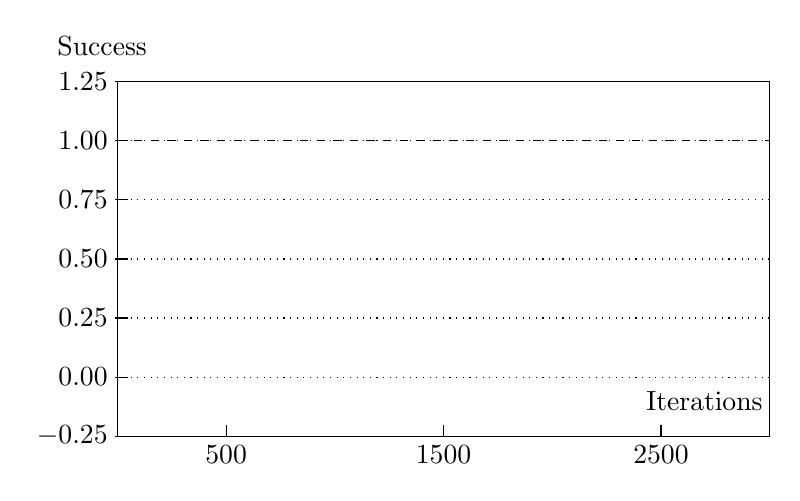
\begin{tikzpicture}[x=0.00276cm,y=3cm]
    % Draw the axes and grid lines
    \draw[-] (0,-0.25) -- (0,1.25) -- (3000,1.25) -- (3000,-0.25) -- cycle; 
    \draw[-,thin, dotted, ystep=0.25, xstep=3000] (0,-0.25) grid (3000,1.25);
    \foreach \x in {500, 1500, 2500}  \draw [-,xshift=0,yshift=-0.25](\x,-0.20) -- (\x,-0.25);
    \foreach \y in {-0.25,0.00,0.25,0.50,0.75,1.00,1.25}  \draw [-,yshift=0](4pt,\y) -- (-1pt,\y);
    \foreach \x/\xtext in {500/500, 1500/1500, 2500/2500} \node at (\x,-0.25) [below] {$\xtext$};
    \foreach \y/\ytext in {-0.25,0.00,0.25,0.50,0.75,1.00,1.25}  \node at (0,\y) [left] {$\ytext$};
    \node at (-70,1.4) {Success};
    \node at (2700,-0.1) {Iterations};
    \draw[-,red] plot[mark=x,mark size=4,mark options={color=red}] 
			file {figs/data/test05v3gmt.CP.tikzdata};
    \draw[-,blue] plot[mark=o,mark size=2,mark options={color=blue}] 
			file {figs/data/test05v3gmt.SP.tikzdata};
    % Also draw the expected convergence: 0.9^8 actions=0.43046
    \draw[dashed,-,yshift=0](0,1.0) -- (3000,1.0);

\end{tikzpicture}

   \caption{Performance of $\CLSELB$ (solid crosses) compared against $\CLSELA$ and $\BULSELA$ (both in dotted grey) in structure $\T_2$ using an applicability threshold of $0.2$.}
   \label{fig:performance-applicability}
\end{figure}


The above results show that the coverage-based confidence weighting can improve
the performance of the \CL\ approach in those cases where it performed poorly due
to false negative experiences, i.e., failure runs for a plan that includes
successful executions.
% %


Finally, we note that coverage-based selection weights encourage the agent to
explore all available options. This further ensures that all solutions are
systematically found, allowing the agent to decide which solution is optimal
faster. For some domains this may be an important feature.









% %%%%%%%%%%%%%%%%%%%%%%%%%%%%%%%%%%%%%%%%%%%%%%%%%%%%
\section{Extended Framework: Event Types and Recursion}\label{sec:extended}
%%%%%%%%%%%%%%%%%%%%%%%%%%%%%%%%%%%%%%%%%%%%%%%%%%%%


\subsection{Event Types}



\subsection{Recursion}






%%%%%%%%%%%%%%%%%%%%%%%%%%%%%%%%%%%%%%%%%%%%%%%%%%%%
\section{The BDI Learning Framework}\label{sec:framework}
%%%%%%%%%%%%%%%%%%%%%%%%%%%%%%%%%%%%%%%%%%%%%%%%%%%%

Our learning task may be summarised as follows: \textit{Given past execution data and the current world state, determine which plan to execute next in order to best address the event-goal in question}. In the BDI sense, our task is to learn the context condition of each plan in the goal-plan hierarchy. In this section we describe our BDI Learning Framework that enables such learning. In particular we describe the use of \dt s for learning context conditions, together with the confidence-based probabilistic plan selection that uses the learning output, with a focus on learning with event-goal types and recursive event-goals.

%%%%%%%%%%%%%%%%%%%%%%%%%%%%%%%%%%%%%%%%%%
\subsection{Integrating Decision Trees into Context Conditions for Plans}
%%%%%%%%%%%%%%%%%%%%%%%%%%%%%%%%%%%%%%%%%%

In a BDI system, a plans context condition is a logical formula that is constructed at design time and evaluated against an event-goal at run time to determine if the plan is applicable in the given world state\footnote{Context formulas may reference internal beliefs as well as environment states, and for this study we treat both as inclusive in the world state.}. As reported in \cite{Airiau:IJAT:09}, in order to allow the context condition to be learnt over time, we annotate each plans context formula with a \textit{\dt}\footnote{It is perfectly feasible to combine the existing logical formula with the \dt\ classification, but to aid our understanding of the \dt\ learning in this study we always use an empty initial formula.}. The idea is that the agent starts with some \textit{necessary but possibly insufficient} conditions for each plan (provided by the designer), and over time and in the course of trying various plans in various world states will be able to \textit{refine} each plans context condition using the learnt \dt\ classification of the world states encountered.

The choice of \dt s as the learning module is motivated by several factors. Firstly, \dt s support hypotheses that are a disjunction of conjunctive terms, and since context formulas are generally expressed in this form then \dt s are readily applicable. Secondly, \dt s can be converted to \textit{if-then} rules that are human readable and can therefore be verified by a domain expert. Finally, \dt s are robust against training data that may contain errors. This is specially relevant in a stochastic domain where perfectly applicable plans may nevertheless fail due to unforeseen circumstances.

The input for the \dt\ learning is a training set of data points of the form $[w,o]$, where $w$ is the world state in which the plan was executed and $o$ was the boolean outcome (success or failure). Initially the training set is empty and grows over time as the agent tries the plan in various world states and samples the result. The world state $w$ itself is a set of discrete attributes that together represent the state of affairs. The idea is that over time the \dt\ will learn a classification based purely on the subset of attributes in $w$ that are relevant to the context condition of the plan. 

The attributes in $w$ determine the quality of the final classification, and their number and possible values has a bearing on the size of the training set required to correctly learn the context condition. The choice of attributes to include in the world state $w$ is a design decision and dependent on domain knowledge. Importantly, the attributes in $w$ should be a superset of the necessary and sufficient attributes relevant to the context condition. For instance, for a plan to pick up an object using a robotic arm, \textit{objectSurface} is a relevant attribute, \textit{gripperWet} possibly is, but \textit{dayOfWeek} likely is not. For the purpose of our study we assume that the designer provides a set of all attributes that are considered possibly relevant to the context condition of the plan. In the worst case, this set is the full set of attributes of the world. 

The decision tree inductive bias is a preference for smaller trees. In other words, the induction of \dt s will trade-off some accuracy in classification for compactness of representation. In fact such inductive bias is necessary if the \dt\ is to generalise to as yet unseen world states. Once a \dt\ is induced from the training set, it may be used to classify any new world state $w$. In the strict sense the classification is an outcome $o$ (failure or success). However, several \dt\ implementations including \propername{J48} in \weka\footnote{In our study we use algorithm \propername{J48}, a version of \propername{c4.5} \cite{Mitchell97:ML}, from the \weka\ learning package \cite{weka99}.} annotate a likelihood of class membership (that is indicative of the inductive bias) to the returned classification. For the given world state $w$ then, we treat the returned likelihood of membership to the $success$ class as the expected likelihood of success of the plan.

One source of misclassification in the learnt \dt s is from erroneous training samples collected when a plan fails not because it was a bad choice in the given world state, but because a bad choice was made somewhere in the execution path below it in the BDI goal-plan hierarchy. Previously in \cite{Airiau:IJAT:09} we have shown how \textit{selective recording} of outcomes may be used to overcome this issue.

A second source of misclassification is from the unorthodox use of \dt s in our framework. Note that the typical use of \dt s lies in the \textit{offline} induction from a complete training set. However, in our case training samples are progressively added after each new execution, while all the time the agent makes the best choice given the experience so far. This results in an incomplete training set in the early stages of learning\footnote{Training data is incomplete in the sense that the agent has only collected a portion of the full data set required to learn the correct classification.} leading to misclassification errors. In \cite{Singh:AAMAS10} we show how a measure of confidence in the \dt\ classification based on the \textit{coverage} of the paths \textit{below} the plan in the goal-plan hierarchy may be used \textit{during plan selection} to address this issue (independent of the recording scheme used).

%%%%%%%%%%%%%%%%%%%%%%%%%%%%%%%%%%%%%%%%%%
\subsection{Confidence-based Probabilistic Plan Selection}
%%%%%%%%%%%%%%%%%%%%%%%%%%%%%%%%%%%%%%%%%%

In previous work \cite{Singh:AAMAS10} we introduced a confidence measure in the \dt\ classification based on the notion of \textit{coverage} of the choices below the plan in the BDI goal-plan hierarchy. The idea is that our confidence in a plan's \dt\ increases as more of the possible execution paths below the plan in the goal-plan hierarchy are explored.

\begin{equation*}\label{eqn:coverage}   
\Omega_P(w) = 0.5 + \left[  c_P(w) *  \left( \kappa_P(w) - 0.5 \right)  \right].
\end{equation*}

Equation \ref{eqn:coverage} shows how the final plan selection weight $\Omega_P(w)$ is calculated for a given world state $w$. Initially, the selection weight for a previously unseen world state $w$ takes the default value of $0.5$. Over time, as the various execution paths below the plan are tried in $w$, its coverage $c_P(w)$ increases and the selection weight approaches the value $\kappa_P(w)$ estimated by the plan's \dt.

Given the set of all applicable plans for resolving event-goal $G$ in world state $w$, the \emph{probabilistic plan selection} mechanism chooses a plan $P_i$ with a probability directly proportional to its selection weight $\Omega_{P_i}(w)$. Such selection ensures a balance between the \emph{exploitation} of current know-how and the \textit{exploration} of new choices. Note that typical BDI platforms do offer various advanced mechanisms for plan selection, including plan precedence and meta-level reasoning. However, these mechanisms are pre-programmed and do not take into account the experience of the agent.


%%%%%%%%%%%%%%%%%%%%%%%%%%%%%%%%%%%%%%%%%%
\subsection{Handling Event-Goal Types}
%%%%%%%%%%%%%%%%%%%%%%%%%%%%%%%%%%%%%%%%%%

Recall our previous definition of the learning task: \textit{Given past execution data and the current world state, determine which plan to execute next in order to best address the event-goal in question}. The simplifying assumption in this definition is that the event-goal in question is an \textit{event-goal instance}. In practical BDI systems, it is often the case that a single plan will handle all instances of an \textit{event-goal type}. Furthermore event-goal instance parameters will generally be included in the context logical formula. Our BDI learning framework account presented earlier in \cite{Airiau:IJAT:09} and \cite{Singh:AAMAS10} did not address the issue of learning context conditions for plans that handle event-goal types, and is the subject of this study.

For the purpose of learning context conditions, we treat the event-goal parameters as relevant attributes of the world. As such, the training set then contains samples of the form $[w \cup \varphi,o]$ where the world state $w$ is the initial set of all relevant attributes that represent the state of affairs, $\varphi$ is the set of all event-type parameters, and $o$ is the outcome class (success or failure). This way, incorporating $\varphi$ in the training data is the only step required for handling event-goal types and no change to the actual framework is warranted.

%%%%%%%%%%%%%%%%%%%%%%%%%%%%%%%%%%%%%%%%%%
\subsection{Support for Recursive Event-Goals}
%%%%%%%%%%%%%%%%%%%%%%%%%%%%%%%%%%%%%%%%%%

Recursion in the context of event-goals refers to the case where the resolution of an event-goal instance $G[\varphi_1]$ involves first the resolution of another goal-event instance $G[\varphi_2]$ of the same type. The result is a growing stack of pending $G[\varphi_i]$ event-goals that eventually terminate in $G[\varphi_n]$ whose parameters satisfy the termination conditions i.e. where a non-recursive plan choice is made.

In order to better understand the impact of recursion on context learning, we use the notion of an \textit{execution trace} that is a sequence of the form $G_0\langle\varphi_0\rangle[P_0:w_0] \cdot G_1\langle\varphi_1\rangle[P_1:w_1] \cdot \ldots \cdot G_n\langle\varphi_1\rangle[P_n:w_n]$, that represents a sequence of event-goals along with the plans selected to handle them and the world state in which the selections were made. So $G_i\langle\varphi_i\rangle[P_i:w_i]$ captures the case where plan $P_i$ was selected in world state $w_i$ in order to achieve the goal-event $G_i\langle\varphi_i\rangle$.

\begin{figure}[t]
\begin{center}
\resizebox{0.8\textwidth}{!}{
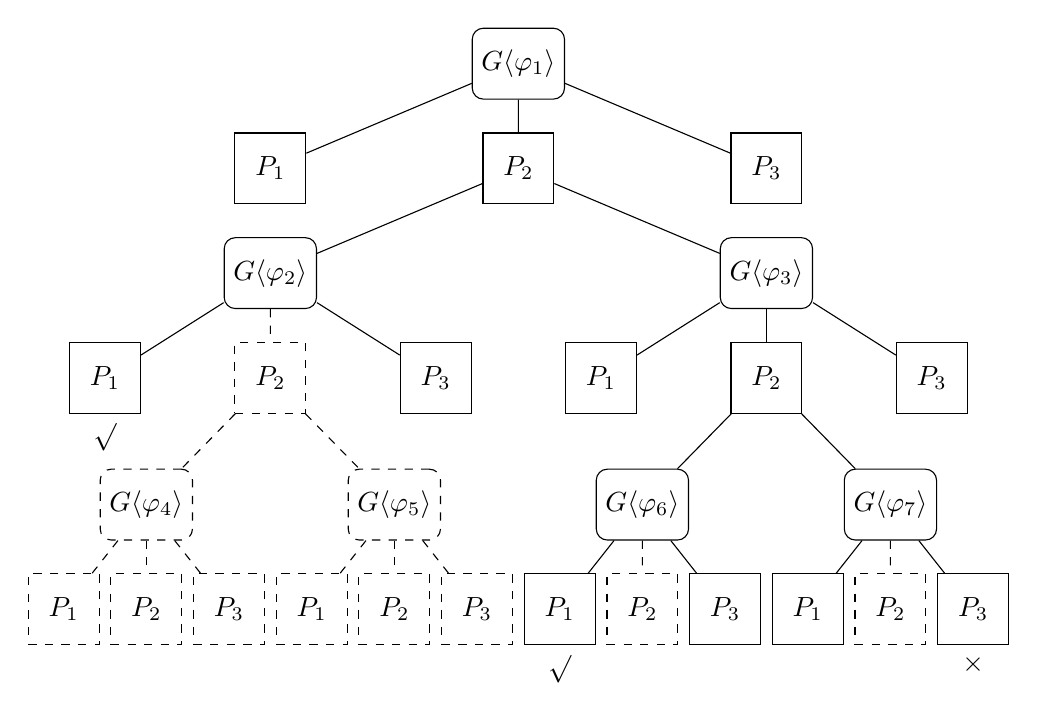
\begin{tikzpicture}[scale=0.7]
\tikzstyle{txt}=[scale=1.0]
\tikzstyle{succ}=[label=below:$\surd$]
\tikzstyle{fail}=[label=below:$\times$]
\tikzstyle{planbox}=[draw,minimum height=0.9cm,minimum width=0.9cm]
\tikzstyle{goalbox}=[draw,rounded corners,minimum height=0.9cm,minimum width=1.0cm]
\tikzstyle{level 1}=[sibling distance=4.5cm,level distance=1.9cm] 
\tikzstyle{level 2}=[sibling distance=9.0cm,level distance=1.9cm] 
\tikzstyle{level 3}=[sibling distance=3.0cm,level distance=1.9cm]
\tikzstyle{level 4}=[sibling distance=4.5cm,level distance=2.3cm]
\tikzstyle{level 5}=[sibling distance=1.5cm,level distance=1.9cm]
\tikzstyle{level 6}=[sibling distance=1.3cm,level distance=1.9cm]

\node[goalbox,yshift=1cm] {$G\langle\varphi_1\rangle$}
	child {node[planbox] {$P_1$}}
	child {node[planbox] {$P_2$}
		child {node[goalbox] {$G\langle\varphi_2\rangle$}
			child {node[planbox,succ] {$P_1$}}
			child[dashed] {node[planbox] {$P_2$}
				child {node[goalbox] {$G\langle\varphi_4\rangle$}
					child {node[planbox] {$P_1$}}
					child {node[planbox] {$P_2$}}
					child {node[planbox] {$P_3$}}
				}
				child {node[goalbox] {$G\langle\varphi_5\rangle$}
					child {node[planbox] {$P_1$}}
					child {node[planbox] {$P_2$}}
					child {node[planbox] {$P_3$}}
				}
			}
			child {node[planbox] {$P_3$}}
		}
		child {node[goalbox] {$G\langle\varphi_3\rangle$}
			child {node[planbox] {$P_1$}}
			child {node[planbox] {$P_2$}
				child {node[goalbox] {$G\langle\varphi_6\rangle$}
					child {node[planbox,succ] {$P_1$}}
					child[dashed] {node[planbox] {$P_2$}}
					child {node[planbox] {$P_3$}}
				}
				child {node[goalbox] {$G\langle\varphi_7\rangle$}
					child {node[planbox] {$P_1$}}
					child[dashed] {node[planbox] {$P_2$}}
					child {node[planbox,fail] {$P_3$}}
				}
			}
			child {node[planbox] {$P_3$}}
		}
	}
	child {node[planbox] {$P_3$}}
;

\end{tikzpicture}

}
\end{center}
\caption{Goal-plan hierarchy $\T_2$ containing a single goal type $G\langle\rangle$ handled by three plans $P_1$, $P_2$ and $P_3$. Here plan $P_2$ posts two instances of $G\langle\rangle$ resulting in recursion. Two levels of recursive unfolding are shown. Dashed $P_2$ nodes indicate roots of unexplored recursive sub-trees.}
\label{fig:unfolding}
\end{figure}

Consider the example BDI goal-plan hierarchy $\T_2$ of Figure \ref{fig:unfolding}. The structure has just a single event-goal type $G\langle\rangle$ and three options to handle it, one of which ($P_2$) in turn posts two instances of the same event-goal type $G\langle\rangle$. In this way, the only plans that take an action in the environment are $P_1$ and $P_3$. The figure highlights an execution trace as follows: \[
\lambda=G\langle\varphi_1\rangle[P_2:w_1] \cdot G\langle\varphi_2\rangle[P_1:w_1] \cdot G\langle\varphi_3\rangle[P_2:w_2] \cdot G\langle\varphi_6\rangle[P_1:w_2] \cdot G\langle\varphi_7\rangle[P_3:w_3].
\]

The first choice in the execution results in the selection of plan $P_2$ to handle event-goal instance $G\langle\varphi_1\rangle$ in a given world $w_1$. Plan $P_2$ in turn immediately posts the event-goal instance $G\langle\varphi_2\rangle$ that is successfully handled by the non-recursive node $P_1$. Plan $P_2$ then posts the second event-goal instance $G\langle\varphi_3\rangle$, which then is handled by itself in a recursive manner.  The outcome is that $\lambda$ traces a path that involves the successive execution of leaf plan $P_1$ for event-goal $G\langle\varphi_2\rangle$ followed by another execution of $P_1$ this time for event-goal $G\langle\varphi_6\rangle$, and finally terminates in the failure of leaf plan $P_3$ for event-goal $G\langle\varphi_7\rangle$. 

Note that if plan $P_2$ had instead been selected to handle $G\langle\varphi_7\rangle$ then a deeper recursive call would have ensued. Similarly if earlier in the execution trace plan $P_2$ was selected to handle event-goal $G\langle\varphi_2\rangle$ then a different recursive sub-tree (shown in Figure \ref{fig:unfolding} as dotted nodes under $G\langle\varphi_2\rangle$) would have unfolded.

The immediate implication of a recursive goal-plan structure is that the size of the hierarchy is no longer static but instead unfolds in a dynamic manner. The issue stems from the fact that the recursion is \textit{unbounded} because the context conditions that cause the recursion to terminate are initially unknown. So in order to know the context conditions we must recursively explore, but in doing so we risk an infinite recursive call because the context conditions that ought to guide the recursive exploration towards termination are unknown. This means that we may never find the ``bottom'' or leaf nodes. This has implications for any \textit{bottom-up} strategies. For instance, our conservative recording approach of \cite{Airiau:IJAT:09} and the coverage-based confidence measure of \cite{Singh:AAMAS10} both suffer from this problem. Interestingly, the simpler aggressive recording approach is not impacted by recursion as it does not consider the goal-plan structure . 

We will now focus on how the coverage-based confidence measure of \cite{Singh:AAMAS10} may be extended for use in recursive hierarchies.

\subsubsection{Calculating Coverage for Recursive Structures}

Since coverage is concerned with the number of paths {below} a plan in the goal-pplan hierarchy, then one way to interpret this for recursive structures is to treat all recursive goals simply as sub-trees in a static structure. Conceptually, this recursive unfolding of the structure is perfectly compatible with the coverage notion. 

Consider again the goal-plan structure $\T_2$ in Figure \ref{fig:unfolding} that shows the unfolding of the hierarchy for two levels of recursion. For the purpose of coverage calculations in this case, the three plans under each goal-event $G\langle\varphi_{4\ldots7}\rangle$ can be seen as having $[1,1,1]$ paths, plans under event-goals $G\langle\varphi_{2\ldots3}\rangle$ as having $[1,9,1]$ paths, and finally plans under $G\langle\varphi_1\rangle$ as having $[1,121,1]$ paths below.

The first difficulty with this reasoning, however, is that in fact the actual number of recursive unfoldings possible starting at $G\langle\varphi_1\rangle$ (or any other $G\langle\rangle$ for that matter) are \textit{infinite}. The only reason we are able to compute paths for structure $\T_2$ is because we have $bounded$ the recursion to a maximum of two levels.

It follows then that wherever a recursive structure applies and the coverage-based confidence measure is to be used, then a maximum recursion value must always be supplied. This may not be an unrealistic given that the domain expert will usually have some idea of how much recursion is sufficient, and as long as they provide a value that is sufficiently large for the domain then we have a valid case for computing coverage.

A second difficulty in this treatment of coverage is that the number of paths is exponential in the recursion number. For instance, in structure $\T_2$ in Figure \ref{fig:unfolding} the number of paths below $P_2$ for a progressively increasing recursion number is the series $[1, 9, 121, 15129, 228947161, \ldots]$. So within four levels of recursion, the number of paths below $P_2$ exceeds $228$ million.

Dhirendra says: Hmm.. one way to handle recursion would be to treat all recursive plans as \textit{leaf} nodes. This will enable coverage and stability to function in recursive domains ``as is''. Also all previous claims about coverage/stability will be preserved. Maybe this treatment of recursion makes more sense than bounded unfolding?!?

%Simplifications: Only single level goal recursion allowed ie G1->P1->G1 and not  G1->P1->G2->P2->G. Also no information of Gs in the system so only the parent goal recursion is tracked.

%\subsubsection{Discussion}
%Can we calculate $c_P(w,r)$ for any r if we have witnessed one r? 

%!TEX root = ../hycas2010.tex
%%%%%%%%%%%%%%%%%%%%%%%%%%%%%%%%%%%%%%%%%%%%%%%%%%%%
\section{A Case Example: The Hanoi Towers Robot}\label{sec:hanoi}
%%%%%%%%%%%%%%%%%%%%%%%%%%%%%%%%%%%%%%%%%%%%%%%%%%%%

\newcommand{\entity}[1]{\texttt{#1}}

To evaluate our learning framework we consider an existing BDI program
from the \JACK\ agent platform
distribution~\cite{BusettaRHL:AL99-JACK}.
% %
The example involves a robot playing the well-known Towers of Hanoi game where the goal is to stack discs of decreasing size onto a single pin. The rules of the game forbid discs to be moved onto smaller discs, however top discs may be moved onto discs of larger size across three pins. The problem is interesting for our purposes since the example solution makes use of event-goal types and recursion. Furthermore, unlike our previous evaluations \cite{Airiau:IJAT:09,Singh:AAMAS10} with synthetic plan libraries, here the evaluation criteria is clear: \emph{does our learning framework achieve the performance of the existing system?}

%Although this is a fairly simple scenario, it is enough to test our overall
%framework. In particular, the plan library makes uses of (goal) recursion and
%events are parametrized. Moreover, even solving a sub-goal such as ``move disc
%$n$ to pin $1$'' may involve many sub-goal postings and plan activations.
%% %
%More importantly, unlike our previous empirical evaluations reported in
%\cite{Airiau:IJAT:09,Singh:AAMAS10} where plan-libraries were ``syntetic'' and
%thus with no special meaning, here we use an \emph{existing} working domain.
%Hence, the evaluation criteria is now more clear: \emph{is our learning framework
%able to achieve the performance of the existing system?}

%The Towers of Hanoi application included in the \JACK\ distribution is as
%follows.
% %
The example solution consists of a \entity{Player} agent that solves the game for 
any given legal initial configuration. The game solving strategy is encoded in plan
\entity{DiscStacker} that solves for one disc at a time starting from the largest
and ending with the smallest onto a chosen pin. This in turn is achieved by posting 
event \entity{Solve(?d,?p)} for solving disc \entity{?d} 
onto pin \entity{?p}. There are four plans that are relevant for this purpose:
% %
%The agent top-level goal is to build the tower of discs in pin number $2$, which
%is captured by the BDI event \entity{BuildTower}.
% %
%To handle such goal event, the agent uses a simple strategy encoded in plan
%\entity{DiscStacker}: stack the discs one by one in pin $2$, starting from the
%largest disc (disc $n$) and ending with he smallest disc (disc $1$). Each disc
%stacking is realized by the (successful) achievemnt of a sub-goal event
%\entity{Solve(?d,?p)}: move disc \entity{?d} to pin \entity{?p}.
%
%Event \entity{Solve(?d,?p)} is indeed the most interesting and complex one. To
%resolve such event, the agent has four plans at disposal that it can use, namely:

\begin{description}

\item[\entity{SolveRight}] This plan solves moving a disc to the pin it is
already on. Since the goal is already true, the plan does \emph{nothing}.

\item[\entity{SolveTopMove}] This plan moves the disc \entity{?d} to the destination
pin \entity{?p} if the disc is not already there and if the move is legal. The actual move
is perfomed by the primitive action \entity{move(?p2,?p)}, where \entity{?p2} is the source pin
of disc \entity{d}.

\item[\entity{SolveTop}] This plan solves for the case when the disc \entity{?d} 
may be legally lifted but cannot be legally placed at the destination because the 
top disc on the destination pin is smaller than \entity{?d}.
% %
In this case, the plan first moves all the discs in the destination pin that are
smaller than disc \entity{?d} to the third (auxiliary) pin, and then
re-posts the sub-goal to move \entity{?d} to pin \entity{?p} i.e. \entity{Solve(?d,?p)}. 

\item[\entity{SolveMiddle}] This plan solves moving a disc from the
\emph{middle} of a stack.
%%
In this case, the plan first clears the source pin so
that disc \entity{?d} becomes the new top of the pin. This is done by
solving for sub-goal \entity{Solve(?d2,?p2)} where disc \entity{?d2} is the
disc currently on top of \entity{?d} and \entity{?p2} is the
auxiliary.
%%
Subsequently the plan re-posts the
sub-goal of moving \entity{?d} to pin \entity{?p} i.e. event \entity{Solve(?d,?p)}.
\end{description}


\begin{figure}[t]
\begin{center}
\resizebox{.9\textwidth}{!}{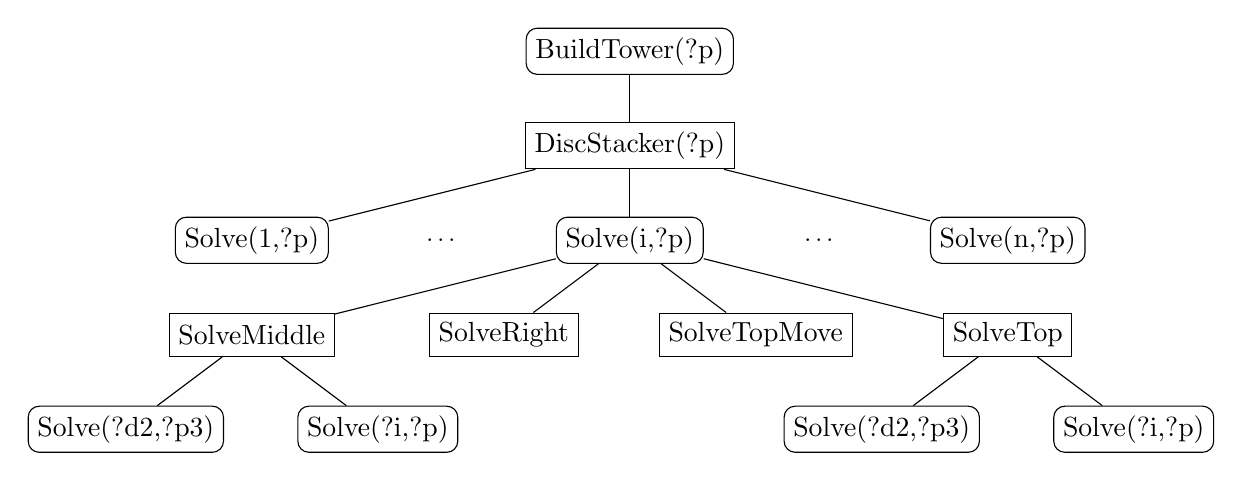
\begin{tikzpicture}[scale=0.8,level distance=1.1cm]
\tikzstyle{txt}=[scale=.9]
\tikzstyle{succ}=[label=below:$\surd$]
\tikzstyle{fail}=[label=below:$\times$]

\tikzstyle{planbox}=[draw,minimum height=0.55cm,minimum width=0.55cm]
\tikzstyle{goalbox}=[draw,rounded corners,minimum height=0.55cm,minimum width=0.55cm]

	
\tikzstyle{level 1}=[sibling distance=4.0cm,level distance=1.5cm] 
\tikzstyle{level 2}=[sibling distance=6cm] 
\tikzstyle{level 3}=[sibling distance=4cm]
\tikzstyle{level 4}=[sibling distance=4cm]
\tikzstyle{level 5}=[sibling distance=3cm]



\node[goalbox,yshift=1cm,solid] (T) {\entity{BuildTower(?p)}}
	child[solid] {node[planbox] {\entity{DiscStacker(?p)}}
		child {node[goalbox] (G1) {\entity{Solve(1,?p)}}}
		child {node[goalbox] (Gi) {\entity{Solve(i,?p)}}
			child {node[planbox] {\entity{SolveMiddle}}
				child {node[goalbox] {\entity{Solve(?d2,?p3)}} }
				child {node[goalbox] (Pi) {\entity{Solve(?i,?p)}} }
			}
			child {node[planbox] {\entity{SolveRight}}}
			child {node[planbox] {\entity{SolveTopMove}}}
			child {node[planbox] {\entity{SolveTop}}
				child {node[goalbox] {\entity{Solve(?d2,?p3)}} }
				child {node[goalbox] {\entity{Solve(?i,?p)}} }
			}
		}
		child {node[goalbox] (Gn) {\entity{Solve(n,?p)}}}
	};
\node[txt] at ($ (G1)!.5!(Gi) $) {$\ldots$};
\node[txt] at ($ (Gi)!.5!(Gn) $) {$\ldots$};
\end{tikzpicture}



}
\end{center}
\caption{Goal-plan hierarchy for the Towers of Hanoi domain.}
\label{fig:hanoi_goalplan}
\end{figure}


Figure~\ref{fig:hanoi_goalplan} illustrates the goal-plan hierarchy for the domain. 
Here we focus on learning the recursive typed \entity{Solve(?d,?p)} event for which we remove the context conditions from the example plans and apply our framework.
% %
%We only show the structure below a \entity{Solve(?d,?p)} goal event once, for the
%case when the plan \entity{Disckstacker} is moving the $i$-th disc to destination
%pin \entity{?p}; all the other instances of such goal have the same form.
% %
%First, notice that this plan-library relies on parametric events. Second, it
%substantially appeals to recursion, in that in order to solve a
%\entity{Solve(?d,?p)} goal event, some strategies use such same event type as a
%sub-goal, namely, strategies \entity{SolveMiddle} and \entity{SolveTop}.
%%
%Observe that the first sub-goals in such plans are relative to some disc
%\entity{?d2} and pin \entity{?p3} that are computed by the plan. For example,
%in plan \entity{SolveMiddle} disc \entity{?d2} is the disk that is currently on
%top of disk \entity{i} and \entity{?p3} is the third pin different from
%destination \entity{?p} and the pin where \entity{i} is located.
%
%Now, clearly, the existing application does include \emph{correct}
%context conditions in each of the plans. So, the context condition of plan
%\entity{SolveRight} states that the current pin location of the disc
%\entity{?d} to be moved is indeed the destination pin \entity{?p}. Similarly,
%plan \entity{SolveTop} states that there is a disc that is smaller than disc
%\entity{?d} in destination pin \entity{?p}.

%So, the first step in our experiment involved \emph{deleting} all preconditions
%from plans. Then, initially, each plan is, in principle, always feasible. The aim
%is that the agent, after experimenting enough in the domain, will eventually
%\emph{learn} the preconditions of each plan.
%% %
%Two problems arise when plans were stripped out of their original context
%conditions.
%% %
%First, some plans may become non ``self-sufficient,'' in that their logic relied
%on variables obtained in the context condition. We solve this by requiring that
%the body programs of plans are indeed self-sufficient: they must be executable
%just by themselves. If the actual body of a plan relies on variables obtained
%while computing the context condition, then the plans themselves must include
%such computations (e.g., obtaining the disc that is on top of the disc to be
%moved).

%The second problem is that plans may succeed in their execution \emph{without}
%actually realizing the goal they have been called for. For instance, suppose that
%plan \entity{SolveRight} is used to resolve goal \entity{Solve(3,2)}, that disc
%\entity{3} is in pin \entity{1} and that disc \entity{5} is at the top of such
%pin. The program of  \entity{SolveRight} simply states to move the disc at the
%top of pin \entity{1} (where the disc to be moved is located) to the destination
%pin, in this case, pin \entity{2}. If pin \entity{2} allows that move, then the
%action \entity{move(1,2)} would succeed and so would plan \entity{SolveRight}.
%However, the goal of concern has not been achieved since all that we have done is
%move disc \entity{5} to pin \entity{2}; disc \entity{3} would still be in pin
%\entity{1}. Note that this will not occurr in the original plan-library because
%its precondition would not hold: disc \entity{3} is \emph{not} at the top of its
%pin.
%% %
%To overcome this problem, we require that every plan includes as its final step a
%test condition for the actual goal to be achieved. See that such test is fully
%determined by the event goal corresponding to the plan. In our case, the last
%step of all four plans for event \entity{Solve(?d,?p)} would be testing that,
%indeed, disc \entity{d} is in pin \entity{p}.

\subsection{Experimental Setup} \label{sec:setup}

The aim of this study is to evaluate our learning framework for recursive event-types. For this reason our experimentation with the Hanoi problem focusses on learning to resolve the recursive event \entity{Solve} only and not on learning the strategy that solves the full Hanoi towers problem (this is done by \entity{DiscStacker(?p)}). Since the full set of possible \entity{Solve} events and initial pin configurations is large, our first step is to construct a sufficiently rich subset that we will use to evaluate our learning approaches. 

We proceed by running the original Hanoi program for a number of randomly generated \entity{Solve} events. For each run we record the \entity{Solve} event, the initial pins configuration, and the maximum recursion encountered for the solution. This gives us a bag of several initial configurations for each recursion level that is a subset of all possible configurations. 

Next, we run each candidate approach on the set of saved configurations for a given recursion level. i.e. where all solutions lie exactly at the specified recursion number. We use a fixed random generation seed for each experiment so that the same sequence of \entity{Solve} events is generated for each learning approach. This isolates any environmental factors and allows us to attribute any differences in performance to the learning approaches alone.

%Finally, since in the Hanoi case we do not care about continuing exploration once a solution is found (optimality of solution is not a requirement), we have implemented two optimisations to the plan selection that boost the selection of plans with known solutions. Firstly, for a given plan, the confidence calculation of Equation \ref{eqn:confidence} is performed only when no solution has previously been found for the given world state, otherwise full confidence is temporarily assumed for that plan. In addition, the plan selection mechanism of Equation \ref{eqn:weight} uses confidence only when no plan has a high expectation of success ($\kappa_P(w) > 0.95$) with high confidence ($c_P(w) > 0.95$), otherwise full confidence is temporarily assumed for \textit{all} plans. 

\subsection{Results}

The following results are for a Hanoi problem with $five$ discs\footnote{We use five discs in order to keep the state space rich enough yet sufficiently small to allow learning runs to be completed and evaluated in reasonable time.}. Each plans domain complexity decay factor for the confidence calculation of Equation \ref{eqn:confidence} are set to $\delta_{Pd} = 0.9$. For goal-plan tree complexity we use $\delta_{Pt} =1$ for non-recursive plans and $\delta_{Pt} =\left[1-(1/r^k)\right]$ for recursive plans where $r$ is the run-time recursion level and $k$ is a scaling factor. Currently, both $\delta_{Pd}$ and $k$ are arbitrarily selected for the domain\footnote{In future work we hope to establish principles for determining general parameters.}. In all experiments, the recursion is bound to a maximum of $eight$ levels that is sufficient to solve all configurations for a five-disc Hanoi problem. The performance of two learning configurations is contrasted. The baseline learning algorithm \CL\ refers to the original aggressive learning approach of \cite{Airiau:IJAT:09} and \cite{Singh:AAMAS10} using the original probabilistic plan selection function that has no confidence-based bias (uses \dt\ expectation of success only). The new algorithm is referred to as \CL+$\Omega$ and uses the same aggressive learning approach as the former but combined with the new confidence-based probabilistic selection function (Equation \ref{eqn:weight}) presented in this study.

\begin{figure*}[t]
\begin{center}
\subfigure[\CL]{\label{fig:result-levelsA}
%!TEX root = ../hycas2010.tex
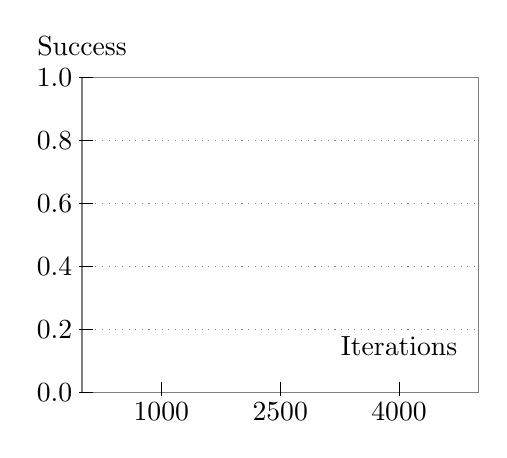
\begin{tikzpicture}[x=0.001cm,y=4cm]
    % Draw the axes and grid lines
    \draw[-,gray] (0,0) -- (0,1) -- (5000,1) -- (5000,0) -- cycle; 
    \draw[-,gray,thin, dotted, ystep=0.2, xstep=5000] (0,0) grid (5000,1);
    \foreach \x in {1000, 2500, 4000}  \draw [-,xshift=0](\x,4pt) -- (\x,-1pt);
    \foreach \y in {0.0,0.2,0.4,0.6,0.8,1.0}  \draw [-,yshift=0](4pt,\y) -- (-1pt,\y);
    \foreach \x/\xtext in {1000/1000, 2500/2500, 4000/4000} \node at (\x,0) [below] {$\xtext$};
    \foreach \y/\ytext in {0.0,0.2,0.4,0.6,0.8,1.0}  \node at (0,\y) [left] {$\ytext$};
    \node at (0,1.1) {Success};
    \node at (4000,0.15) {Iterations};
    \draw[-,gray] plot[mark=+,mark size=4,mark options={color=black}] 
			file {data/hanoid5s1r8.CP.tikzdata};
    \draw[-,gray] plot[mark=o,mark size=3,mark options={color=black}] 
			file {data/hanoid5s3r8.CP.tikzdata};
    \draw[-,gray] plot[mark=x,mark size=4,mark options={color=black}] 
			file {data/hanoid5s5r8.CP.tikzdata};

\end{tikzpicture}

}
\qquad
\subfigure[\CL+$\Omega$]{\label{fig:result-levelsB}
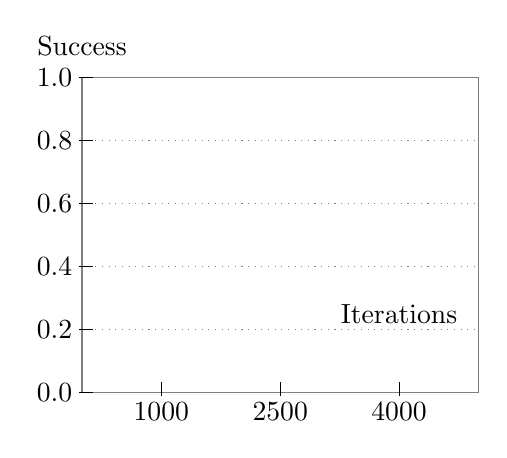
\begin{tikzpicture}[x=0.001cm,y=4cm]
    % Draw the axes and grid lines
    \draw[-,gray] (0,0) -- (0,1) -- (5000,1) -- (5000,0) -- cycle; 
    \draw[-,gray,thin, dotted, ystep=0.2, xstep=5000] (0,0) grid (5000,1);
    \foreach \x in {1000, 2500, 4000}  \draw [-,xshift=0](\x,4pt) -- (\x,-1pt);
    \foreach \y in {0.0,0.2,0.4,0.6,0.8,1.0}  \draw [-,yshift=0](4pt,\y) -- (-1pt,\y);
    \foreach \x/\xtext in {1000/1000, 2500/2500, 4000/4000} \node at (\x,0) [below] {$\xtext$};
    \foreach \y/\ytext in {0.0,0.2,0.4,0.6,0.8,1.0}  \node at (0,\y) [left] {$\ytext$};
    \node at (0,1.1) {Success};
    \node at (4000,0.25) {Iterations};
    \draw[-,gray] plot[mark=+,mark size=4,mark options={color=black}] 
			file {data/hanoid5s1r8.CF.tikzdata};
    \draw[-,gray] plot[mark=o,mark size=3,mark options={color=black}] 
			file {data/hanoid5s3r8.CF.tikzdata};
    \draw[-,gray] plot[mark=x,mark size=4,mark options={color=black}] 
			file {data/hanoid5s5r8.CF.tikzdata};

\end{tikzpicture}

}
\caption{Agent performance under \CL\ and \CL+$\Omega$ schemes for solutions at recursion levels one (pluses), three (circles) and five (crosses). Each point represents results from $5$ experiment runs using an averaging window of $100$ samples.}
\label{fig:result-levels}
\end{center}
\end{figure*}

To understand how the two approaches perform for solutions of varying difficulty we conducted a set of experiments with solutions at different recursive levels. Each experiment consisted of resolving a known set of \entity{Solve} event configurations, saved earlier as described in Section \ref{sec:setup}, whose solutions all required a given recursive depth. Figure \ref{fig:result-levels} shows that as the solution difficulty increases from one to five recursion levels, \CL\ performance drops much more significantly compared to that of \CL+$\Omega$. For instance, for solutions requiring five levels of recursion, \CL\ achieves only $50\%$ success at $5k$ iterations whereas \CL+$\Omega$ achieves $95\%$ success by $3.5k$ iterations. The poor performance of \CL\ may be attributed to the fact that deeper solutions require more \entity{move(?p2,?p)} steps and where an earlier success does not exist to guide selection at each resulting state the exploration is mostly random. On the other hand, the confidence-based measure of Equation \ref{eqn:weight} takes into account the goal-plan tree complexity and is able to guide the \CL+$\Omega$ exploration towards the deeper solutions.

Next, we conducted an experiment that consisted of resolving the full set of saved \entity{Solve} events i.e. the set had solutions dispersed through all possible recursion levels. Figure \ref{fig:result-fullA} shows the results for the two approaches where as expected \CL+$\Omega$ performs better than \CL\ overall. For the same experiment, we also recorded the number of solutions found. Figure \ref{fig:result-fullB} shows that \CL+$\Omega$ resolves all $52$ goals within $12k$ iterations whereas \CL\ resolves only $47$ by the end of the experiment at $20k$. At a similar point of comparison, to resolve $47$ goals \CL+$\Omega$ takes around $6.4k$ iterations whereas \CL\ takes more than twice as long at $17.7k$. The vertical dashed lines in Figure \ref{fig:result-fullA} and Figure \ref{fig:result-fullB} mark the $47$th and $51$st solutions.

\begin{figure*}[t]
\begin{center}
\subfigure[Success Rate]{\label{fig:result-fullA}
../../../writeup/2010HYCAS/figs/result-fullA.tex
}
\qquad
\subfigure[Solutions Found]{\label{fig:result-fullB}
%!TEX root = ../hycas2010.tex
% Points in the input file are y-scaled by 0.5 so yval 1000 represents point 2000 in the original results. The reason for scaling was that TeX cannot handle > ~16k numbers
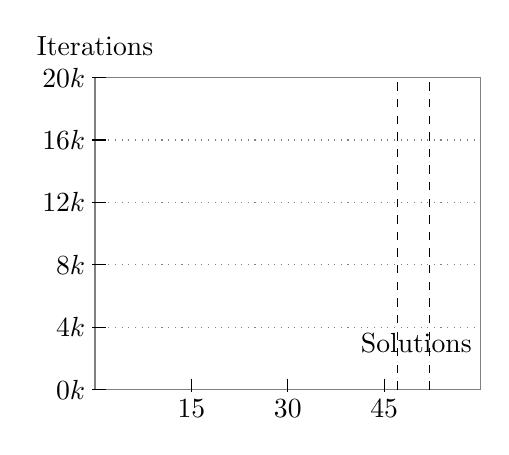
\begin{tikzpicture}[x=0.0816cm,y=.0004cm]
    % Draw the axes and grid lines
    \draw[-,gray] (0,0) -- (0,10000) -- (60,10000) -- (60,0) -- cycle; 
    \draw[-,gray,thin, dotted, ystep=2000, xstep=60] (0,0) grid (60,10000);
    \foreach \x in {15, 30, 45}  \draw [-,xshift=0](\x,4pt) -- (\x,-1pt);
    \foreach \y in {0,2000,4000,6000,8000,10000}  \draw [-,yshift=0](4pt,\y) -- (-1pt,\y);
    \foreach \x/\xtext in {15/15, 30/30, 45/45} \node at (\x,0) [below] {$\xtext$};
    \foreach \y/\ytext in {0/0k,2000/4k,4000/8k,6000/12k,8000/16k,10000/20k}  \node at (0,\y) [left] {$\ytext$};
    \node at (0,11000) {Iterations};
    \node at (50,1500) {Solutions};
    \draw[-,gray] plot[mark=o,mark size=3,mark options={color=black}] 
			file {data/hanoi5s.CP.tikzdata};
    \draw[-,gray] plot[mark=x,mark size=4,mark options={color=black}] 
			file {data/hanoi5s.CF.tikzdata};
	\draw [-,dashed](47,0pt) -- (47,10000);
	\draw [-,dashed](52,0pt) -- (52,10000);
\end{tikzpicture}

}
\caption{Agent performance under \CL\ (circles) and \CL+$\Omega$ (crosses) schemes. Each point represents an average result from $5$ experiment runs.}
\label{fig:result-full}
\end{center}
\end{figure*}

Finally, we ran a third experiment to understand the impact of applicability thresholds. In the classical BDI framework plans are either applicable or not in a boolean decision. However, in our modified framework plans are applicable according to the selection weight given by Equation \ref{eqn:weight}. Since plan execution is often not cost-free in real systems, it is likely that an adequate plan selection scheme would not select \textit{any} plan if they all have too low an expectation of success, and an agent may fail a plan without even trying. To represent this scenario we setup an applicability threshold of $20\%$ whereby plans with expectations of success less than this threshold would not be selected. In this case \CL\ shows a complete inability to learn as reported earlier \cite{Singh:AAMAS10}. In contrast \CL+$\Omega$ benefits from the adjusted selection weights of Equation \ref{eqn:weight} and shows similar performance as before (Figure \ref{fig:result-fullA})\footnote{The threshold of $0.2$ while somewhat arbitrary is consistent with that used earlier \cite{Singh:AAMAS10}. The difference between the default weight ($0.5$) and the threshold weight ($0.2$ in this case) decides how much ``give'' we have in the exploration. The closer the threshold is to $0.5$ the greater the chance that the plan will be aborted before a solution is found.}.

%A final observation in Figure \ref{fig:result-full} is that neither approach converges to $1.0$. This is because the Hanoi domain is not free from goal inter-dependence. So if a plan learns to solve a sub-goal in two ways that each lead to different end states, then depending on the way the sub-goal was resolved the top level goal may pass or fail. Indeed, when we analyse the result log we find that \CL+$\Omega$ finds all solutions as expected, but even so fails now and then for some of these because of the way a sub-goal was realised. Our learning framework does not currently support goal inter-dependence.

A final observation in Figure \ref{fig:result-fullA} is that \CL+$\Omega$ does not reach the performance of the hand-crafted JACK program and converges to about $90\%$ success even though it successfully discovers all solutions.
This is because the decision tree representation does not guarantee that the training data will always be correctly classified (we discuss this accuracy versus compactness trade-off in Section \ref{sec:decision_trees}). For instance, a decision tree may report a poor likelihood of success for a given state even when the associated training sample indicates success, due to the sample being misclassified in the failure ``class''. The only way to guarantee correctness would be to use the training data directly, for instance using a look-up table. Furthermore, when the learnt decision trees are converted to rules they do not ``look'' like the original ones but are far more complex. This is mainly due to representational differences as our simple representation is propositional whereas the original conditions are relational.



%%%%%%%%%%%%%%%%%%%%%%%%%%%%%%%%%%%%%%%%%%%%%%%%%%%%
\section{Discussion and Conclusion}\label{sec:discussion}
%%%%%%%%%%%%%%%%%%%%%%%%%%%%%%%%%%%%%%%%%%%%%%%%%%%%

In this paper we propose a technique to enhance the typical plan selection
mechanism in BDI systems by allowing agents to learn and adapt the context
conditions of existing plans in the agent's plan library.
%%
As designing adequate context conditions that take full account of the agent's
environment for its complete life-cycle is often non-trivial, a framework that
allows for the \emph{refinement} of (initial) context conditions of plans
\textit{based on experience} is desirable. To this end we extend the BDI
framework to use \dt{}s as (part of) context conditions and provide a
probabilistic plan selection mechanism that caters for both exploration and
exploitation of plans.


We empirically evaluate two approaches to learning context conditions from experience, an aggressive approach that records and uses every outcome for learning, and a more conservative approach that records failure outcomes only when it considers the preceding choices that led to failure to be well-informed.
We confirm results from \cite{APSS08} that each approach has advantages in certain situations, but highlight an important shortcoming of the aggressive approach --- its complete inability to learn when applicability thresholds are used i.e. when the agent abandons plans with low chances of success. We then show that a new plan selection mechanism that also accounts for our confidence in the \dt\ classification can overcome the earlier issues with the aggressive approach. We conclude that the aggressive approach (that is also simpler), combined with the confidence measure (that also provides flexibility for tuning to different situations) is a better candidate for the general setting.

Our experiments do not consider the effects of conflicting interactions between sub-goals of a plan. For instance, if a sub-goal could succeed in more than one way causing different changes in the environment, one of which may in fact cause a subsequent sub-goal to fail, then in our current implementation it is not possible to detect and learn such interactions. Similarly we do not currently consider the effects of using failure recovery, under which alternative plans are tried upon the failure of a plan for achieving a goal. We note that both these features should be resolved for the real system. Moreover, we plan to do further experimentation with more realistic programs from existing applications. For continuous attributes, our approach requires that either the attributes be discretized or additional discrete attributes be used to test the continuous ones (for instance, check if temperature is $<20.5\textcelsius$).

One critique of the coverage-based confidence measure used is that it has a defined end state ($c_T(S)=1$) whereas for a real system, learning and re-learning will occur indefinitely as the agent continually tries to adapt to a changing environment. This implies that our confidence in a \dt's classification would also require calibration based on a changing environment. If the change in the environment was deliberate, then our confidence could be reset and subsequently \textit{re-built}. Without such an explicit signal the agent must rely on other methods for determining when the environment has changed significantly.

An appealing measure for recognising environmental changes is through the relatedness of its features. For instance, an observation that the grass is \textit{wet} presumably has a high correlation to the fact that it is \textit{raining}, and a \dt\ may (based on prior observations) very well use these factors in determining the likelihood of success of a plan to navigate the field. If then, we were to witness a world where it is not raining but the grass is wet (could be morning dew), then this world would be very different from the typical worlds we have seen so far and so we may have strong reason to reduce our confidence in the \dt\ classification of this new world.

The issue of combining learning and deliberative approaches for decision making in autonomous systems has not been widely addressed. In \cite{Riedmiller01} learning is used prior to deployment for acquiring low level robot soccer skills that are then treated as fixed methods in the deliberative decision making process once deployed. Hern\'andez et al. \cite{Hernandez04:Learning} give a preliminary account of how decision trees may be induced on plan failures in order to find an alternative logical context conditions in a deterministic paint-world example. More recently, in work related to BDI systems, \cite{Zhuo09:Learning} propose a method for learning hierarchical task network (HTN) method preconditions with partial observations in more complex domains. For this they first construct constraints from observed decomposition trees that are then solved offline using a constraint solver. In our work, learning and deliberation is integrated (as in \cite{APSS08}) such that one impacts the other and the classical exploration/exploitation dilemma applies. Initially, instead of following a random exploration policy (as is the case for agents with no initial knowledge), our agents are guided by the existing domain knowledge inherent in the BDI hierarchy.





%% The Appendices part is started with the command \appendix;
%% appendix sections are then done as normal sections
%% \appendix

%% \section{}
%% \label{}

%% References
%%
%% Following citation commands can be used in the body text:
%% Usage of \cite is as follows:
%%   \cite{key}         ==>>  [#]
%%   \cite[chap. 2]{key} ==>> [#, chap. 2]
%% 

%% References with bibTeX database:

\bibliographystyle{elsarticle-num}
\bibliography{hycas2010}

%% Authors are advised to submit their bibtex database files. They are
%% requested to list a bibtex style file in the manuscript if they do
%% not want to use elsarticle-num.bst.

%% References without bibTeX database:

% \begin{thebibliography}{00}

%% \bibitem must have the following form:
%%   \bibitem{key}...
%%

% \bibitem{}

% \end{thebibliography}


\end{document}

%%
%% End of file `elsarticle-template-num.tex'.
